\documentclass{oblivoir}

\usepackage{graphicx}
\usepackage{cleveref}
\usepackage{hyperref}

\newcommand{\figref}[1]{\figurename~\ref{#1}}

\maxtocdepth{subsubsection}
\maxsecnumdepth{subsubsection}

\title{JAVA프로그래밍실습(12746) 학기 과제 보고서}
\author{순천향대학교 SW융합대학 컴퓨터소프트웨어공학과\\20223519 전한결}

\begin{document}

    \maketitle

    \begin{itemize}
        \item 작성자 – SW융합대학 컴퓨터소프트웨어공학과 20223519 전한결
        \item 과목 – 2023학년도 1학기 JAVA프로그래밍실습(12746)
        \item 과제 제시일 – 2023년 3월 13일
        \item 과제 마감일 – 2023년 6월 2일
    \end{itemize}

    \pagebreak

    \tableofcontents

    \pagebreak

    \section{과제 개요}
    \label{sec:overview}

    이 과제는 순천향대학교 SW융합대학 컴퓨터소프트웨어공학과의
    2023학년도 1학기 과목 JAVA프로그래밍(12746), JAVA프로그래밍실습(12746)의
    학기 과제이다.

    이번 과제에서는 음료를 판매하는 자판기를 만들어야 한다.
    여기서 자판기란 프로그램상에서의 가상 자판기이기는 하나,
    실제 자판기에 탑재하여 사용할 수 있을 정도로 실제 상황들을
    구현한 자판기여야 한다.

    과제에서는 실제 자판기에서 사용될 수 있기 위해 필요한 몇가지
    조건들을 제시한다.
    여기에는 재고와 화폐 보관소, 거스름의 구현과, 특정한 상호작용을 통해
    접근할 수 있는 관리자 메뉴 등이 포함되어있다.

    또한 과제 진행에 있어 필수적으로 사용해야 하는 자료구조와
    개발 언어가 결정되어있고,
    개발하는 데에 사용할 라이브러리 등이 권고되어있다.

    이 자판기 프로그램과 함께,
    자판기 프로그램을 만드는 데에 사용한 설계서와 최종 완료 보고서를
    제출하는 것이 이번 과제의 요구 사항이다.

    \subsection{자세한 기능적 요구사항}
    \label{subsec:requirements}

    아래는 기본적으로 요구되는 기능이다.
    \begin{itemize}
        \item 판매하는 음료의 개수는 기본적으로 5개로 하되,
        각각 450원(물), 500원(커피), 550원(이온음료), 700원(고급커피),
        750원(탄산음료)으로 한다 (반드시 클래스 사용).
        \item 각각 음료의 재고는 기본적으로 3개로 하며(생성자로 초기화),
        3개 이상 음료가 배출되었을 때는 해당 음료 (물품)에 대해
        품절 표시를 하고 해당 음료를 더 이상 선택할수 없어야 한다
        \begin{itemize}
            \item 단, 이전에 재고가 보충되었을 경우에는 해당 재고만큼의 판매가 가능해야 함.
        \end{itemize}
        \item 입력 받을 수 있는 화폐의 단위는 10원, 50원, 100원, 500원,
        1,000원으로만 한정하되, 지폐로 입력 받을 수 있는 금액의
        상한선은 3,000원까지이며, 지폐와 동전을 모두 포함하여
        총 5,000원을 초과하여 입력 받을 수 없다
        (화폐의 입력 금액에 따라 판매 가능 음료가 표기되어야 한다).
        \begin{itemize}
            \item 이 때, 화폐를 입력 받는 변수는 반드시
            동적 할당을 통한 레퍼런스화 해야 하며,
            화폐가 반환되거나 음료의 판매가 끝나면
            동적 할당을 해제해야 한다.
        \end{itemize}
        \item 기본적으로 거스름 돈을 가지고 있어야 하며
        (각 동전별로 5개를 기본 값으로 하고 음료의 개수와 마찬가지로
        생성자를 사용하여 초기화 할 것),
        거스름 돈 반환 혹은 음료 판매에 따른 동전의
        가감이 구현되어야 한다.
        또한 음료 자판기에서 화폐를 입력 받을때는 반드시
        사용자 요구에 의한 화폐 반환이 가능해야 한다.
        \item 음료가 배출된 이후에도 반드시 다시 화폐를 입력 받을 수 있는
        상태가 되어야 한다.
        \item 관리자 메뉴 (비밀번호 확인을 통해 관리자 메뉴에 접근할
        수 있도록 작성하되, 비밀번호는 반드시 특수문자 및
        숫자가 하나 이상 포함된 8자리 이상으로 설정할 수 있도록 해야 하며
        필요시 언제든 변경 가능해야 함)는 다음과 같은 조건을 만족해야 한다.
        \begin{itemize}
            \item 일별/월별 매출 산출, 각 음료의 일별/월별 매출,
            각 음료의 재고 보충이 가능해야한다.
            이 때, 일별/월별 매출은 사전에 파일로 저장해 놓은
            파일(각자 만들어 사용)을 사용하여야 하며,
            현재의 자판기 매출은 사전에 저장해 놓은 파일과
            연관성을 가지고있어야 한다.
            \item 관리자 메뉴에서는 현재 자판기 내의 화폐현황을
            손쉽게 파악할 수 있어야 하며,
            관리자가 “수금”이란 메뉴를 선택할 경우,
            해당 금액을 수금할 수 있어야 한다.
            단, 이 경우에도 반환을 위한 최소한의 화폐
            (임의로 지정할 것)는 남겨두어야 한다.
            \item 관리자 메뉴에서는 각 음료의 판매가격,
            판매이름을 사용자의 입력을 통해 언제든 바꿀 수 있어야 한다.
            \item 관리자 메뉴와 관련된 모든 사항들은 파일로
            읽기/쓰기가 되어야 한다.
            (최소 기록 사항: 일별/월별 매출, 재고 소진 날짜 혹은 주기)
        \end{itemize}
        \item 반드시 예외 처리 및 주석 (프로그램, 함수, 라인 주석 등)이
        반드시 포함되어야 한다.
        \item 예외처리시 JAVA 언어의 예외처리 방식에 따른 동작을 사용해야 하며,
        모든 부분에 예외처리가 잘 이루어져야 한다.
        \item 상기한 바와 같은 프로그램의 실행은 모두 GUI 환경에서 동작하여야 한다.
    \end{itemize}

    과제에서는 도전해볼 수 있는 추가적인 요구사항을 제공한다.
    \begin{itemize}
        \item 각 음료의 재고 수량은 Linked-List를 통해 구현되어야 한다.
        \item 본 프로그램의 작성 시 Stack과 Queue가 적절한 곳에
        1회 이상씩 사용되어야 한다.
        \item 본 프로그램의 작성 시 Tree 구조가 적절한 곳에 1회 이상씩
        사용되어야 한다.
        \item 본 프로그램의 작성 시 다양한 Sort 및 Search 기법이
        적절한 곳에 1회 이상씩 사용되어야 한다.
        \item 본 프로그램의 작성 시 스윙 컴포넌트와 스레드가
        적절한 곳에 1회 이상씩 사용되어야 한다.
        \item 본 프로그램에서 작성하는 자판기 관리 프로그램을 통해
        생성/저장된 모든 데이터들은 Socket 프로그래밍을 통해
        지정된 서버로 전송되어 관리될 수 있어야 한다.
        또한 상기한 바와 같은 데이터를 수신한 서버는
        다음과 같은 기능을 수행할 수 있어야 한다.
        \begin{itemize}
            \item 각 자판기의 각 음료별 일별/월별 매출현황의 합산/누적합산
            \item 각 자판기의 일별/월별 매출 현황의 합산/누적합산
            \item 각 자판기의 실시간 재고현황 파악
            \item 각 자판기의 음료 재고 부족 시 관리자에게 알림 메시지 전송
            \item 각 자판기의 음료 이름 변경
            \item 기타
        \end{itemize}
        \item 본 프로그램의 동작은 적어도 3대 이상의 PC
        (Client1, Client2, Server) 혹은 Socket 프로그래밍을 통해
        통신할 수 있는 3가지의 환경에서 동작할 수 있어야 한다.
        \item 기타: 명시된 기능들 외에 자신의 프로그램만의 특장점이 될 수 있는
        기능들을 추가할 경우 이를 명시하고 구현할 수 있다.
    \end{itemize}

    \section{설계}

    이번 장에서는 자판기 프로그램의 설계에 대해 다룬다.
    조건을 만족시키는 자판기 프로그램을 만들기 위하여 필요한 요소들을
    다음과 같이 정리하였다.

    \subsection{상위 설계}

    자판기의 구매자, 관리자를 포함하는 사용자가
    자판기 프로그램(이하 자판기)을 사용할 때에
    어떤 방식으로 사용 경험을 주어주는지에 대한 설계를 진행한다.

    \subsubsection{자판기 화면}

    자판기 화면은 자판기를 음료 구매 목적으로 사용하는 사람들이
    사용하기 위한 화면이다.
    자판기 화면에 있는 내용은 자판기를 실행하면 가장 처음으로 볼 수 있다.

    자판기 화면에서는 다음과 같은 작업을 수행할 수 있다.
    \begin{itemize}
        \item 돈 투입
        \item 음료 구매
        \item 거스름돈 수거
    \end{itemize}

    \subsubsection{관리자 화면}

    관리자 화면은 자판기 관리자를 위한 화면이다.
    자판기 화면에서 관리자 화면을 띄우는 버튼을 누르면
    비밀번호를 입력하고 접속할 수 있다.

    관리자 화면에서는 다음과 같은 작업을 수행할 수 있다.
    \begin{itemize}
        \item 매출 산출
        \item 재고 보충
        \item 재고 확인
        \item 화폐 현황 확인
        \item 화폐 수금
        \item 음료 정보(가격, 이름) 수정
        \item 관리 로그 확인
    \end{itemize}

    \subsubsection{서버 측 관리자 화면}

    서버 측 관리자 화면은 자판기와 연결되어있는
    서버에서 확인할 수 있는 화면이다.
    서버의 구현방법 상 클라이언트(자판기) 측 환경과는 다르게
    CLI로 구현되어있다.

    서버 측 관리자 화면에서는 다음과 같은 작업을 수행할 수 있다.
    \begin{itemize}
        \item 각 자판기의 관리자 화면에서 수행할 수 있는 작업 수행
        \item 자판기에서 발생한 재고, 화폐 부족 등의 알림 확인
    \end{itemize}

    \subsection{상세 설계}

    각 화면에서 수행할 수 있는 작업들을 구현하기 위해
    어떻게 기능을 구현할지 대략적인 설계를 진행한다.

    \subsubsection{자판기 화면}

    \paragraph{화폐 보관함}

    화폐 보관함은 거스름으로 활용되는 현금을 모아놓는 공간이다.
    화폐 보관함에는 10원부터 10,000원까지 각각의 화폐를
    얼마나 사용할 수 있는지에 대한 정보를 담아놓게 되고,
    일정한 액수의 거스름돈을 거슬러줘야 할 때에나
    관리자 화면에서 화폐를 수금할 때 등에 사용한다.

    \paragraph{거스름}

    거스름은 화폐 보관함에 있는 돈의 일부를 사용자에게 반환하는 행위이다.
    거스름은 사용 가능한 단위의 화폐를 최고권부터 순회하여 거슬러야 하는
    금액이 될때까지 거스름돈 목록에 추가한다.
    이 방식을 통하면 최소한으로 적은 개수의 화폐권을 가지도록
    거스름을 처리할 수 있으므로 바람직하다.

    경우에 따라서 거스름을 해야 하는 요금을 거스르지 못할 수도 있다.
    이러한 경우는 크게 거스름돈을 모두 사용해도 거슬러줘야 하는 경우에
    미치지 못하는 경우와 거스름돈으로 사용할 수 있는 화폐권의 종류가
    적절하지 않은 경우로 나눌 수 있다.
    두 가지 경우 모두 자판기를 사용하는 사람으로 하여금 거스름돈을
    부족하게 받게 하므로,
    이러한 경우에는 클라이언트–서버 통신을 통한 로그를 남겨
    추후에 관리자가 직접 잔돈을 처리할 수 있게 하는 것이 바람직하다.

    위와 같은 경우를 미연에 방지하는 것이
    자판기를 사용하는 사람으로 하여금
    사용자 경험을 증대시킬 수 있기 때문에,
    자판기에 돈을 넣기 전에 거스를 수 있는 돈이 일정 액수 이하임을
    알리는 방식으로 사용자에게 주의를 주어야 한다.

    \paragraph{음료 보관함}

    음료 구매를 위해서 음료의 재고를 기록해놓아야 한다.

    음료 보관함에 더 이상의 음료가 없다면 사용자는 음료를
    구매할 수 없다.
    따라서 자판기는 음료를 구매할 수 없을 때에 사용자가 현금을 투입하기 전에
    주의를 주어야 한다.

    재고는 음료의 정보와 개수를 멤버로 하는 객체의 목록으로 저장된다.

    음료의 종류는 5개까지로 한다.
    자판기의 특성상 음료의 종류를 늘리려면 기계의 구조를 변경해야
    하기 때문에 음료의 종류를 가변적으로 설정하는 것은 현실적이지 않다.

    \subsubsection{관리자 화면}

    \paragraph{재고 기록}

    프로그램이 종료되었다가 다시 실행되는 경우에도 직접 동기화하지 않고
    이전 상태를 유지하여 사용할 수 있도록,
    자판기와 사용자의 상호작용 후에는 현재 상태와 상호작용 내용을
    기록해 두어야 한다.

    또한 프로그램이 실행될 때에 재고 기록이 있는지 확인하고,
    없을 때에는 기본 상태로 자판기를 초기화하는 등의 조치도
    관리자의 사용자 경험을 위해 필요하다.

    \paragraph{화폐 수금}

    화폐 수금 시에는 사전에 설정한 개수는 화폐 보관함에 꼭 남아있도록
    설정한다.

    \paragraph{로그}

    로그는 클라이언트에서 서버로 전달하는 등 통신에서 활용할 수 있도록
    JSON이나 xml과 같이 처리가 간편한 방식을 사용한다.
    또한 로그의 종류에 따라 디렉토리를 분리하고 로그가 발생한 시점을
    이름으로 한 파일을 로그별로 따로 저장하여 추후에
    프로그램을 사용하지 않은 디버깅 등이 용이하도록 한다.

    \subsubsection{서버 측 관리자 화면}

    \paragraph{프로토콜}

    서버와 클라이언트가 서로 정보를 주고받기 위한 프로토콜을 제작하여
    오류가 적고 형식이 갖춰진 통신을 수행할 수 있도록 한다.

    \paragraph{로그 확인}

    로그에 대한 확인은 최신 정보를 일정한 개수만큼 로드하는 것으로
    확인할 수 있도록 한다.

    \section{프로토콜}
    \label{sec:protocol}

    자판기의 경우 정보를 만들어내는 것이 자판기 쪽이고,
    언제나 하나의 관리자 클라이언트에 접속되지 않은 상태에서도
    자판기가 작동할 수 있어야 하므로
    자판기 측에 서버를 두고 관리자 클라이언트가 서버---자판기에 접속하여
    정보를 주고받는 방식으로 구현한다.

    프로토콜에서 사용하는 포트 주소는 9832로 한다.

    따라서 아래의 프로토콜은 관리자 클라이언트에서 자판기 서버로
    전송하는 프로토콜이다.

    \subsection{오류 코드}

    \begin{itemize}
        \item 0: OK
        \item 1: 인증 실패
        \item 2: 이어지는 정보
        \item 3: 정보 부족
        \item 4: 통신 종료
        \item 5: 잘못된 명령어
    \end{itemize}

    \subsection{프로토콜 목록}

    \paragraph{AUTH}
    AUTHorize.
    자판기 서버에 관리자로 접속한다.

    \begin{verbatim}
C: AUTH
S: 3 정보 부족
C: AUTH qwerty
S: 1 인증 실패
C: AUTH >Oj1i38aB
S: 0 OK
    \end{verbatim}

    \paragraph{GSEL}
    Get SELls.
    자판기의 매출 정보를 요청한다.

    \begin{verbatim}
C: GSEL
S: 2 2
S: 물 450 3
S: 탄산음료 750 2
    \end{verbatim}

    \paragraph{GINV}
    Get INVentory.
    자판기의 재고 정보를 요청한다.

    \begin{verbatim}
C: GINV
S: 2 5
S: 물 0
S: 커피 3
S: 이온음료 3
S: 고급커피 3
S: 탄산음료 1
    \end{verbatim}

    \paragraph{GLOG}
    Get LOGs. 자판기의 로그 정보를 요청한다.

    \begin{verbatim}
C: GLOG 10
S: 1 인증 실패
C: GLOG
S: 3 정보 부족
C: GLOG 10
S: 2 10
S: 2023-05-25 09:56:17.476 [관리접속] 비밀번호를 사용하여 관리자 콘솔에 로그인하였습니다.
S: 2023-05-25 09:56:31.721 [관리퇴장] 관리자가 콘솔을 닫았습니다.
S: 2023-05-25 09:56:34.783 [현금투입] 1000원 투입. 거스름 버퍼에 1000원 남음 (10*0, 50*0, 100*0, 500*0, 1000*1)
S: 2023-05-25 09:56:37.060 [상품판매] 물통 판매 (30개 남음), 남은 현금 550원
S: 2023-05-25 09:56:39.191 [상품판매] 물통 판매 (29개 남음), 남은 현금 100원
S: 2023-05-25 09:56:41.173 [잔돈반환] 거스름돈을 처리했습니다. 10*0,
50*0, 100*1, 500*0, 1000*0, 거스름돈 버퍼에 0원 남음. 현금 버퍼에는 각각 10, 9, 14, 8, 6개 남음
S: 2023-05-25 09:56:45.435 [관리접속] 비밀번호를 사용하여 관리자 콘솔에 로그인하였습니다.
S: 2023-05-25 09:58:32.489 [관리퇴장] 관리자가 콘솔을 닫았습니다.
S: 2023-05-24 21:56:19.281 [관리접속] 비밀번호를 사용하여 관리자 콘솔에 로그인하였습니다.
S: 2023-05-24 21:56:45.678 [관리퇴장] 관리자가 콘솔을 닫았습니다.
    \end{verbatim}

    \paragraph{SPRD}
    Set PRoDuct.
    자판기의 음료 정보를 설정한다.

    SPRD 뒤에 이어오는 자료는 각각 음료의 인덱스,
    음료의 재고, 음료의 이름이다.

    \begin{verbatim}
C: GINV
S: 2 5
S: 물 0
S: 커피 3
S: 이온음료 3
S: 고급커피 3
S: 탄산음료 1
C: SPRD 3
S: 3 정보 부족
C: SPRD 2 3 사탕
S: 0 OK
    \end{verbatim}

    \paragraph{QUIT}
    QUIT. 자판기 서버와의 접속을 종료한다.

    \begin{verbatim}
C: QUIT
S: 4 통신 종료
    \end{verbatim}

    \paragraph{IATH}
    Is AuTHorized.
    자판기 서버에 관리자로 접속되어 있는지 확인한다.

    \begin{verbatim}
C: IATH
S: 1 인증 실패
C: AUTH >Oj1i38aB
S: 0 OK
C: IATH
S: 0 OK
    \end{verbatim}

    \section{실행 화면}

    \subsection{메인 화면}

    자판기를 실행하면 \figref{fig:vending-machine}\과 같은 화면이 나타난다.
    \begin{figure}[h]
        \centering
        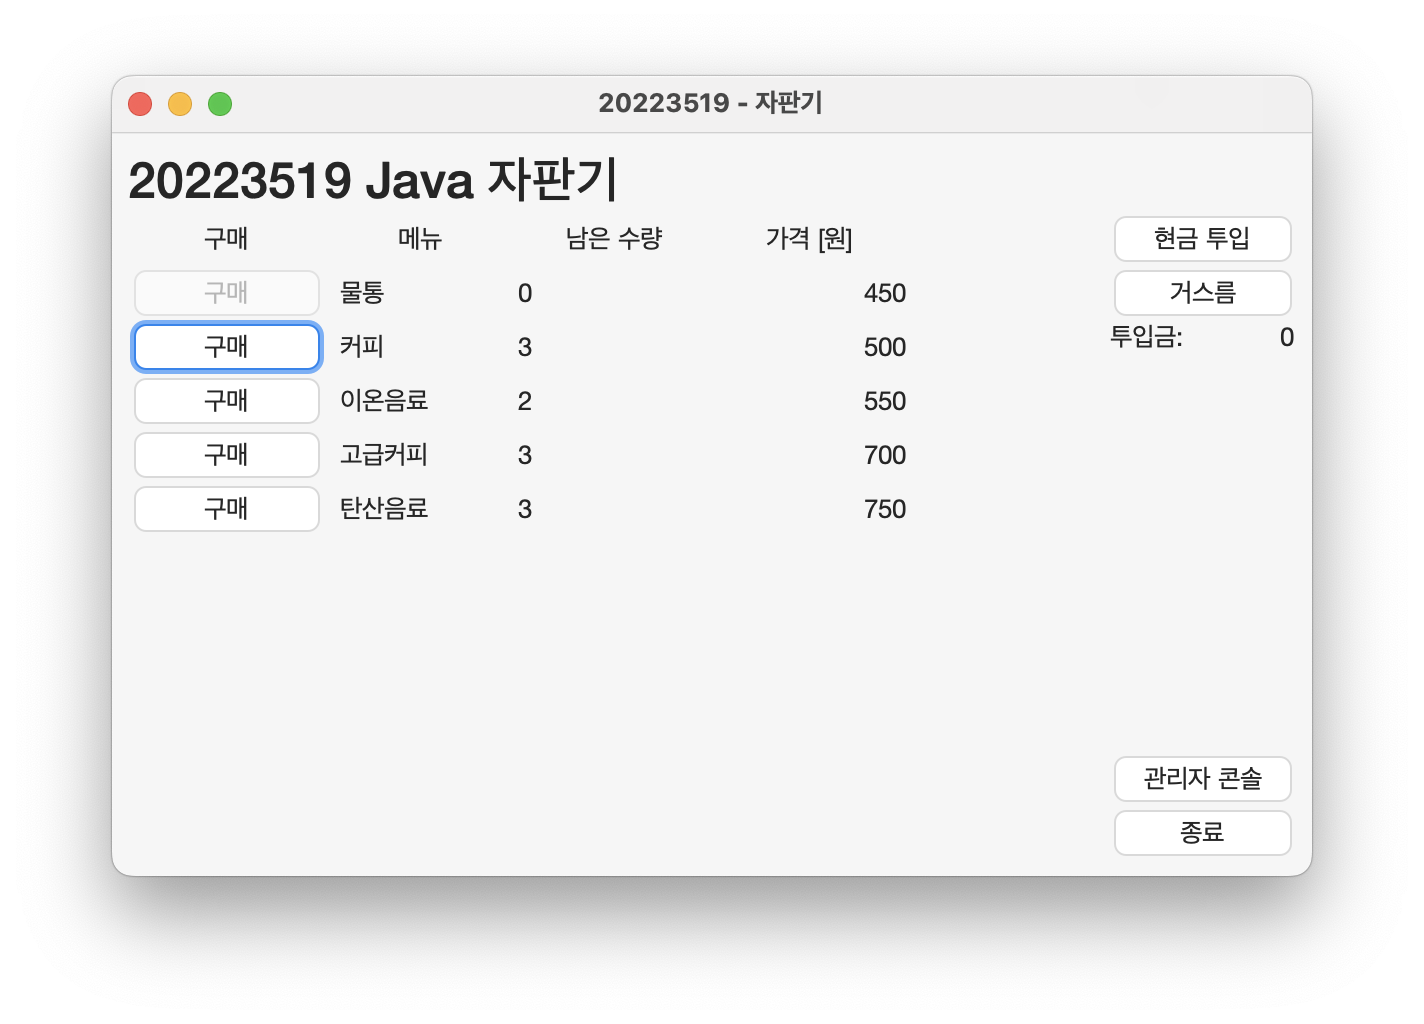
\includegraphics[width=0.5\textwidth]{images/snapshot/vending-machine}
        \caption{자판기의 실행 화면}
        \label{fig:vending-machine}
    \end{figure}

    여기에서는 음료의 목록을 확인할 수 있다.
    음료를 구매하거나, 현금을 투입하거나, 거스름돈을 반환하거나 관리자로 로그인할 수 있다.
    종료 버튼을 누르면 바로 프로그램이 종료된다.

    만약 재고가 없어서 음료를 구매할 수 없는 경우에는 \figref{fig:vending-machine}의 `물통' 구매 버튼과 같이
    비활성화되어 클릭할 수 없게 된다.

    음료를 구매할 때에 잔고가 부족하면 음료를 구매할 수 없다. 이 경우에는 \figref{fig:not-enough}\와 같은 오류 메시지가 표시되며,
    성공적으로 음료가 구매된 경우에는 \figref{fig:bought-coffee}\와 같은 메시지가 표시된다.
    \begin{figure}[h]
        \centering
        \begin{minipage}{.5\textwidth}
            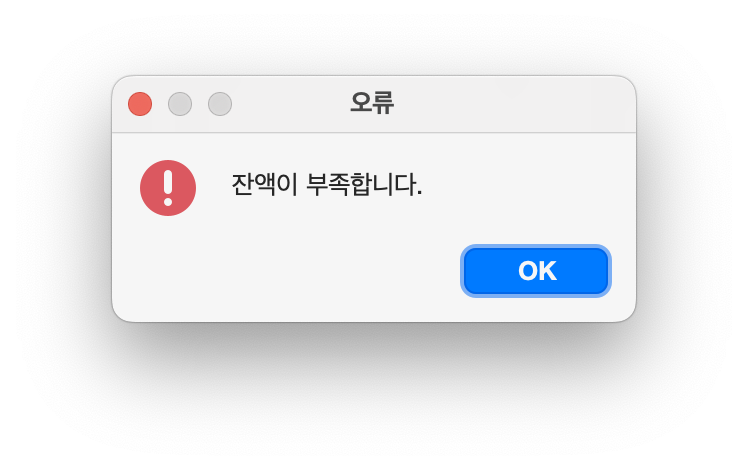
\includegraphics[width=\textwidth]{images/snapshot/not-enough}
            \caption{잔고 부족 오류 메시지}
            \label{fig:not-enough}
        \end{minipage}%
        \begin{minipage}{.5\textwidth}
            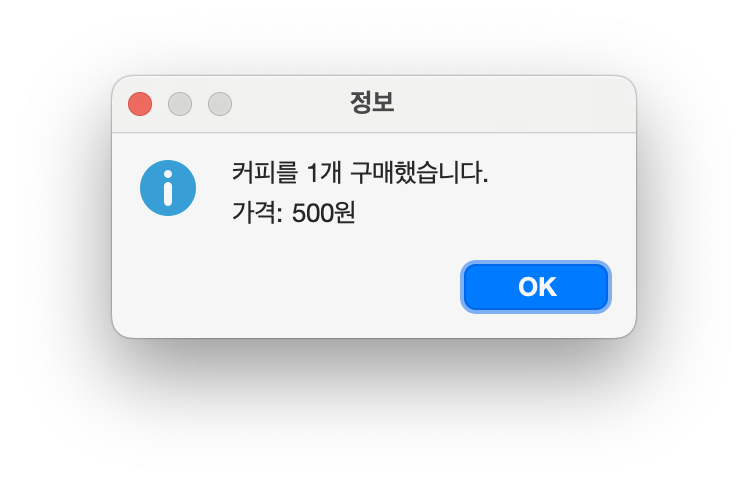
\includegraphics[width=\textwidth]{images/snapshot/bought-coffee}
            \caption{음료 구매 성공 메시지}
            \label{fig:bought-coffee}
        \end{minipage}
    \end{figure}

    현금 투입 버튼을 누르면 \figref{fig:cash-input}\와 같은 화면이 나타난다.
    여기서 투입할 금액을 입력하고 확인 버튼을 누르면 현금이 투입된다.

    거스름 돈 반환 버튼을 누르면 \figref{fig:change}\와 같은 화면이 나타난다.
    \begin{figure}[h]
        \centering
        \begin{minipage}{.5\textwidth}
            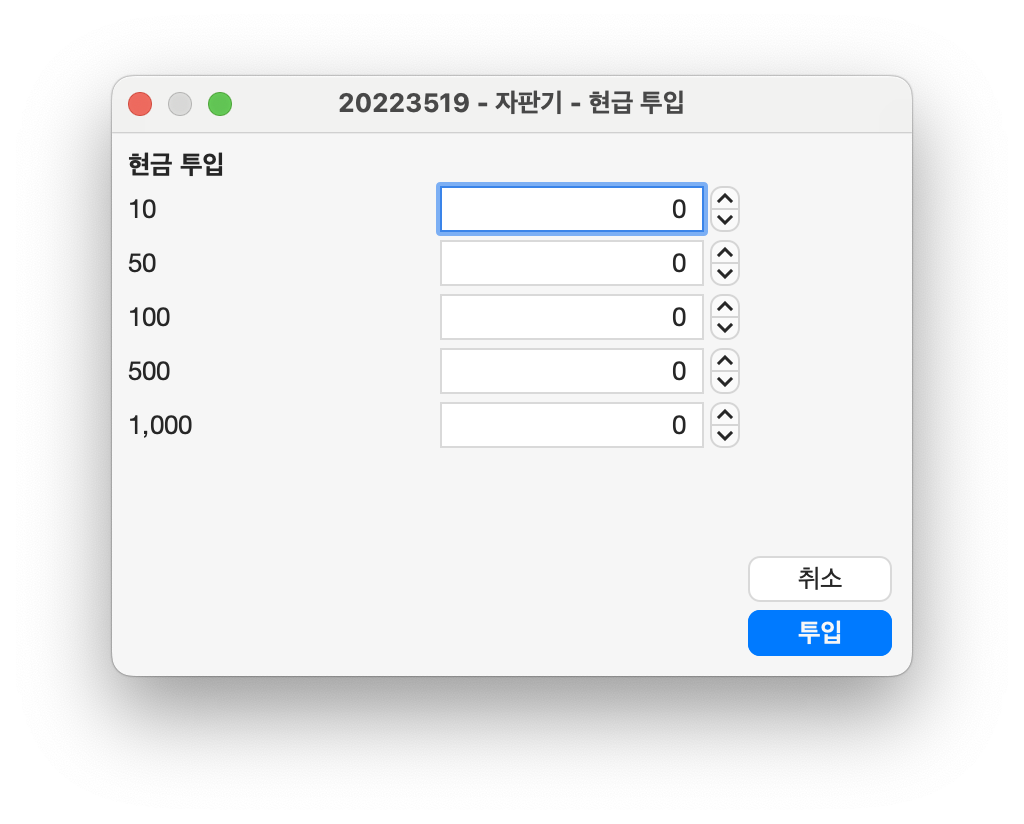
\includegraphics[width=\textwidth]{images/snapshot/cash-input}
            \caption{현금 투입 화면}
            \label{fig:cash-input}
        \end{minipage}%
        \begin{minipage}{.5\textwidth}
            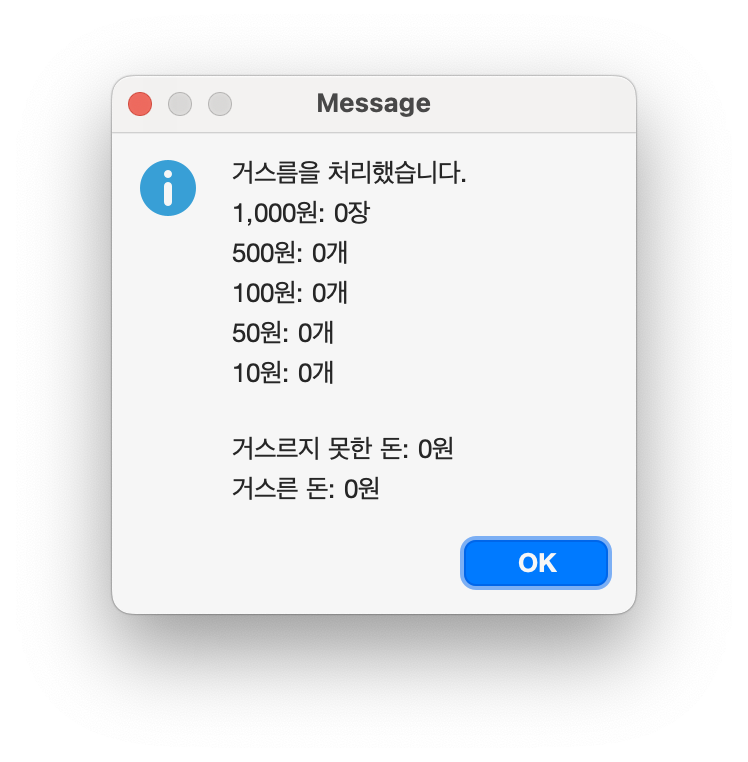
\includegraphics[width=\textwidth]{images/snapshot/change}
            \caption{거스름 돈 반환 화면}
            \label{fig:change}
        \end{minipage}
    \end{figure}
    거스를 돈이 없거나 성공적으로 거스름에 실패한 경우에도 똑같이 \figref{fig:change}\와 같은 화면이 나타난다.

    관리자 콘솔 버튼을 누르면 \figref{fig:password}\과 같은 화면이 나타난다.
    \begin{figure}[h]
        \centering
        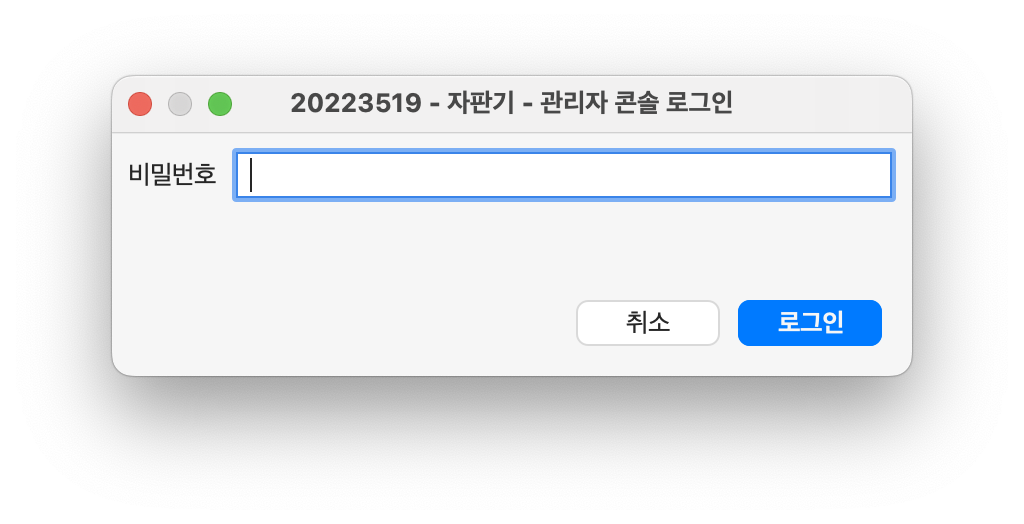
\includegraphics[width=0.5\textwidth]{images/snapshot/password}
        \caption{관리자 콘솔 비밀번호 입력 화면}
        \label{fig:password}
    \end{figure}
    만약 비밀번호가 이미 지정되어있지 않다면 \figref{fig:password-set-0}\와 같이 비밀번호를 설정하는 창이 나타난다.
    비밀번호를 설정하는 창에서는 비밀번호 조건에 맞춰 비밀번호를 설정할 수 있도록 왼쪽 아래에 \figref{fig:password-set-1}\와 같은
    메시지가 표시된다.
    \begin{figure}[h]
        \centering
        \begin{minipage}{0.5\textwidth}
            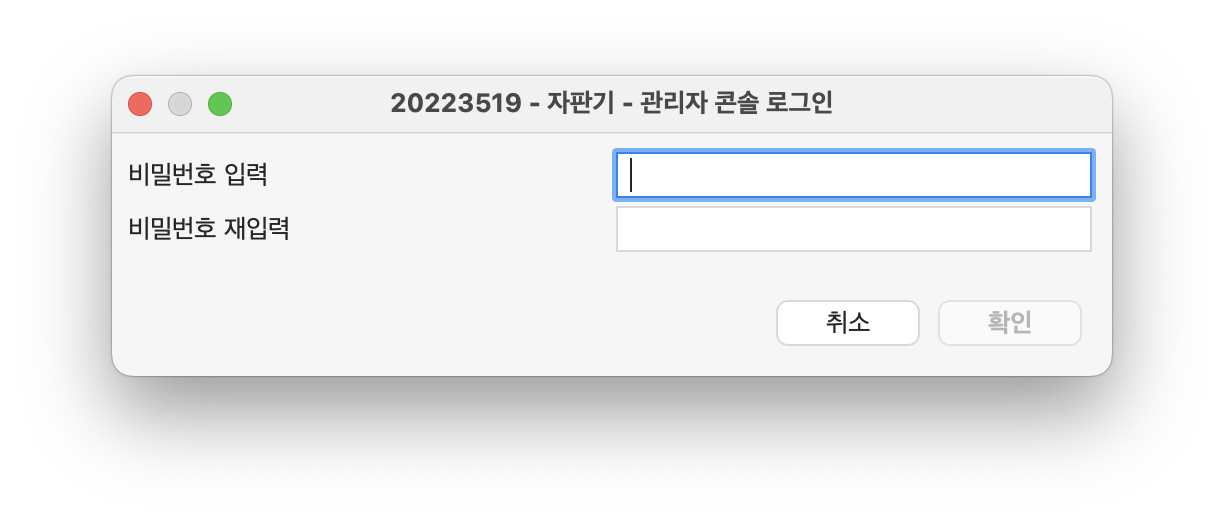
\includegraphics[width=\textwidth]{images/snapshot/password-set-0}
            \caption{관리자 콘솔 비밀번호 설정 화면}
            \label{fig:password-set-0}
        \end{minipage}%
        \begin{minipage}{0.5\textwidth}
            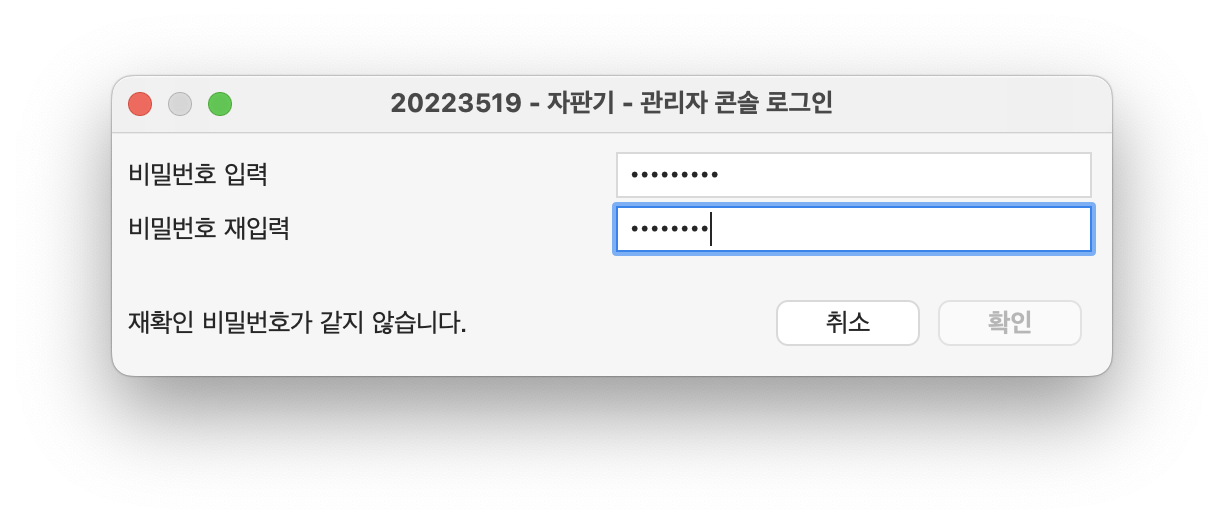
\includegraphics[width=\textwidth]{images/snapshot/password-set-1}
            \caption{관리자 콘솔 비밀번호 설정 화면}
            \label{fig:password-set-1}
        \end{minipage}
    \end{figure}

    성공적으로 비밀번호를 입력하면 관리자 콘솔 화면으로 이동할 수 있다.

    \subsection{관리자 콘솔}

    관리자 콘솔을 처음으로 시작하면 일단 \figref{fig:admin-daily-log}\와 같은 화면에서 일 매출을 확인할 수 있다.
    \begin{figure}[h]
        \centering
        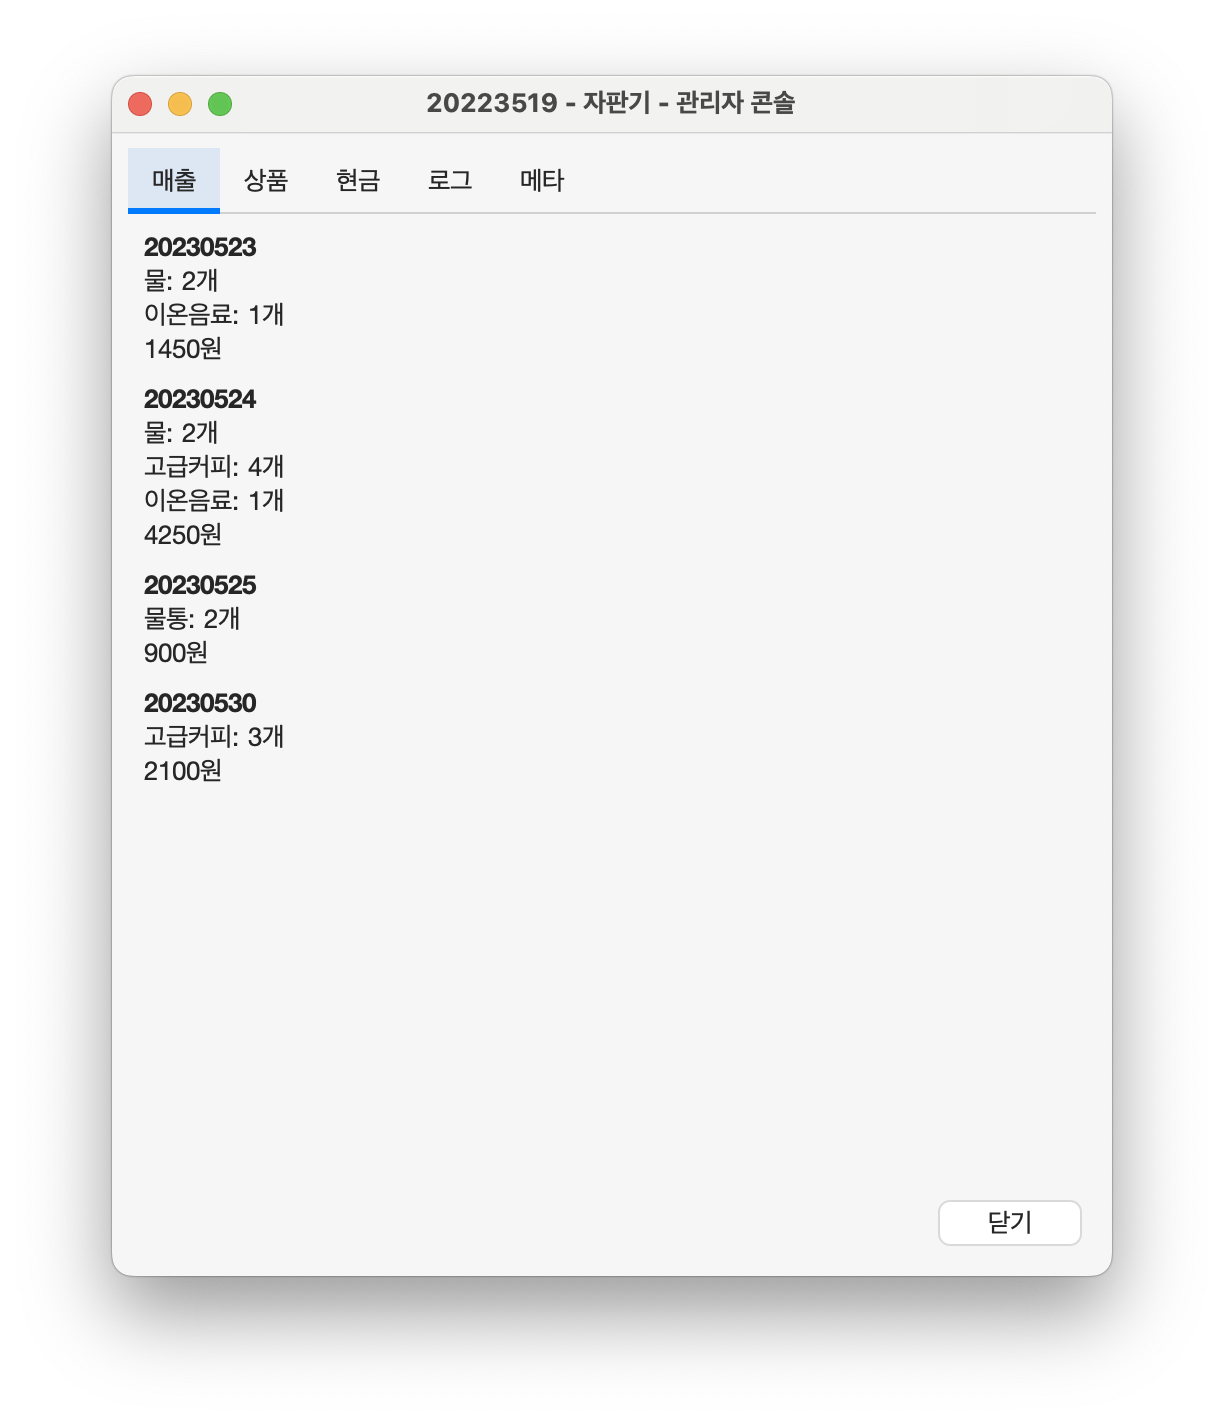
\includegraphics[width=0.5\textwidth]{images/snapshot/admin-daily-log}
        \caption{관리자 콘솔 일 매출 확인 화면}
        \label{fig:admin-daily-log}
    \end{figure}
    각각의 매출은 판매한 음료의 이름과 개수, 그리고 매출액으로 구성되어 있다.

    관리자 콘솔의 상단에는 매출, 상품, 현금, 로그, 메타 탭을 확인할 수 있는데,
    각각은 일별 매출, 상품 관리, 현금 수금, 로그 확인, 메타적인 관리를 위한 탭이다.
    상품 이하의 탭은 \figref{fig:admin-inventory}부터 \figref{fig:admin-meta}\와 같이 구성되어 있다.

    \begin{figure}
        \centering
        \begin{minipage}{.5\textwidth}
            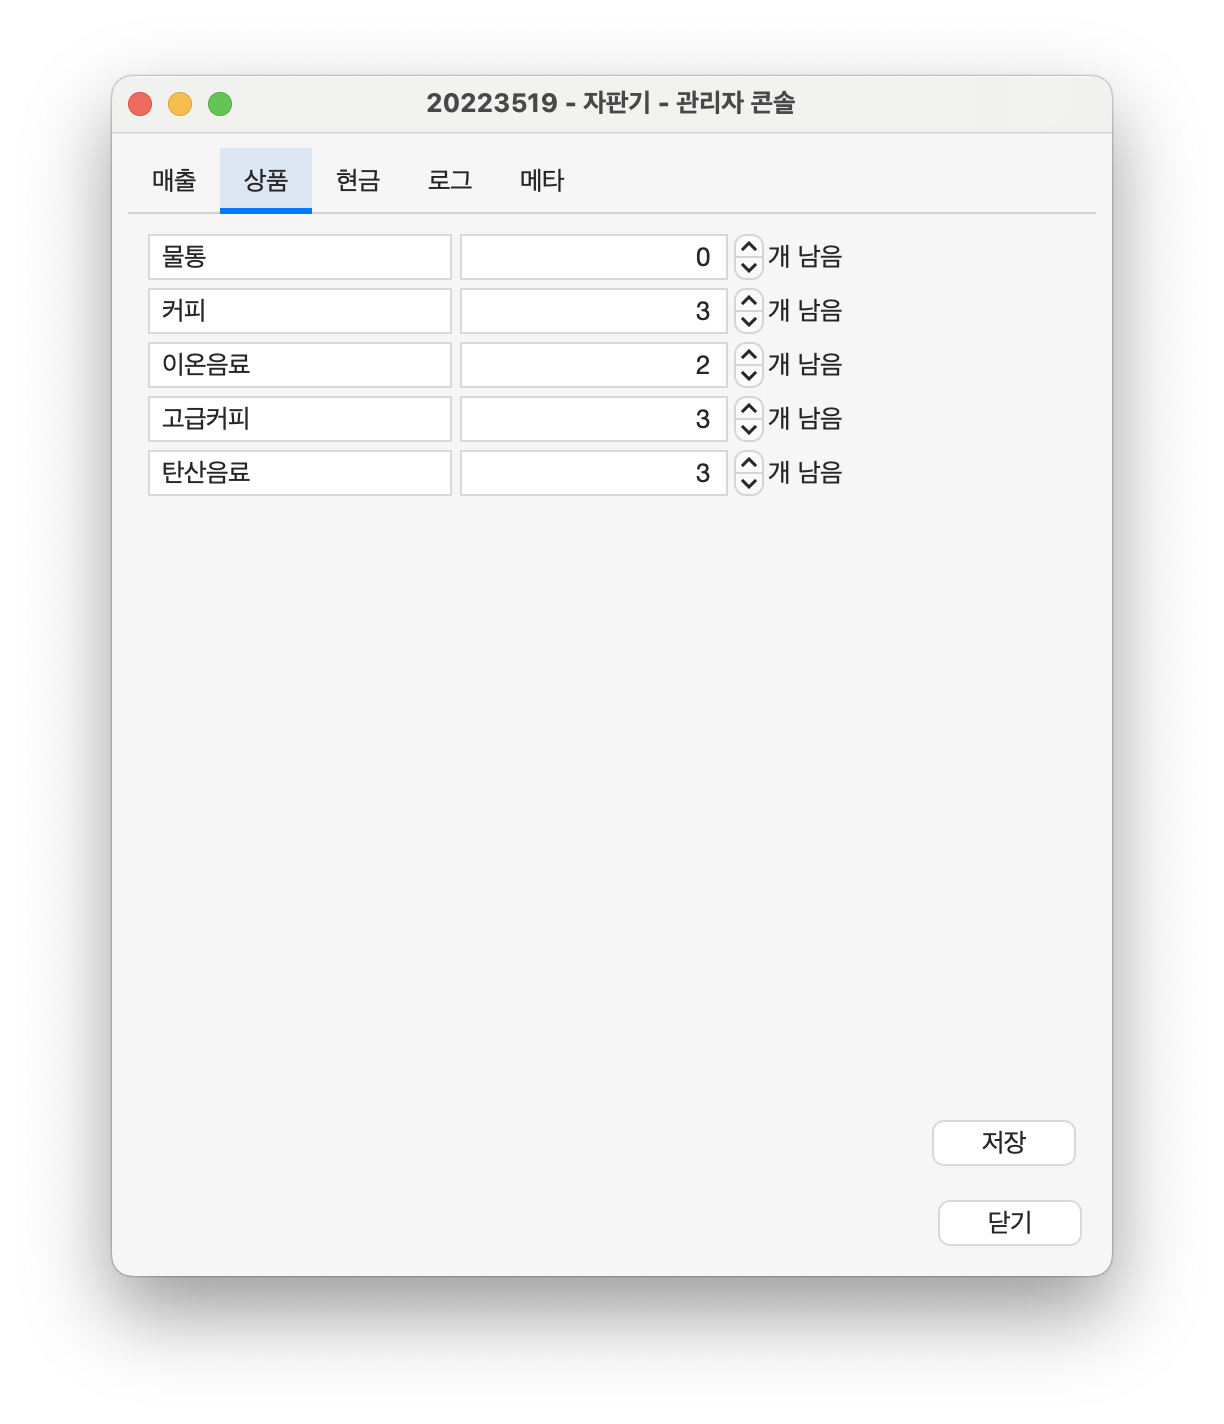
\includegraphics[width=\textwidth]{images/snapshot/admin-inventory}
            \caption{관리자 콘솔 상품 관리 탭}
            \label{fig:admin-inventory}
        \end{minipage}%
        \begin{minipage}{.5\textwidth}
            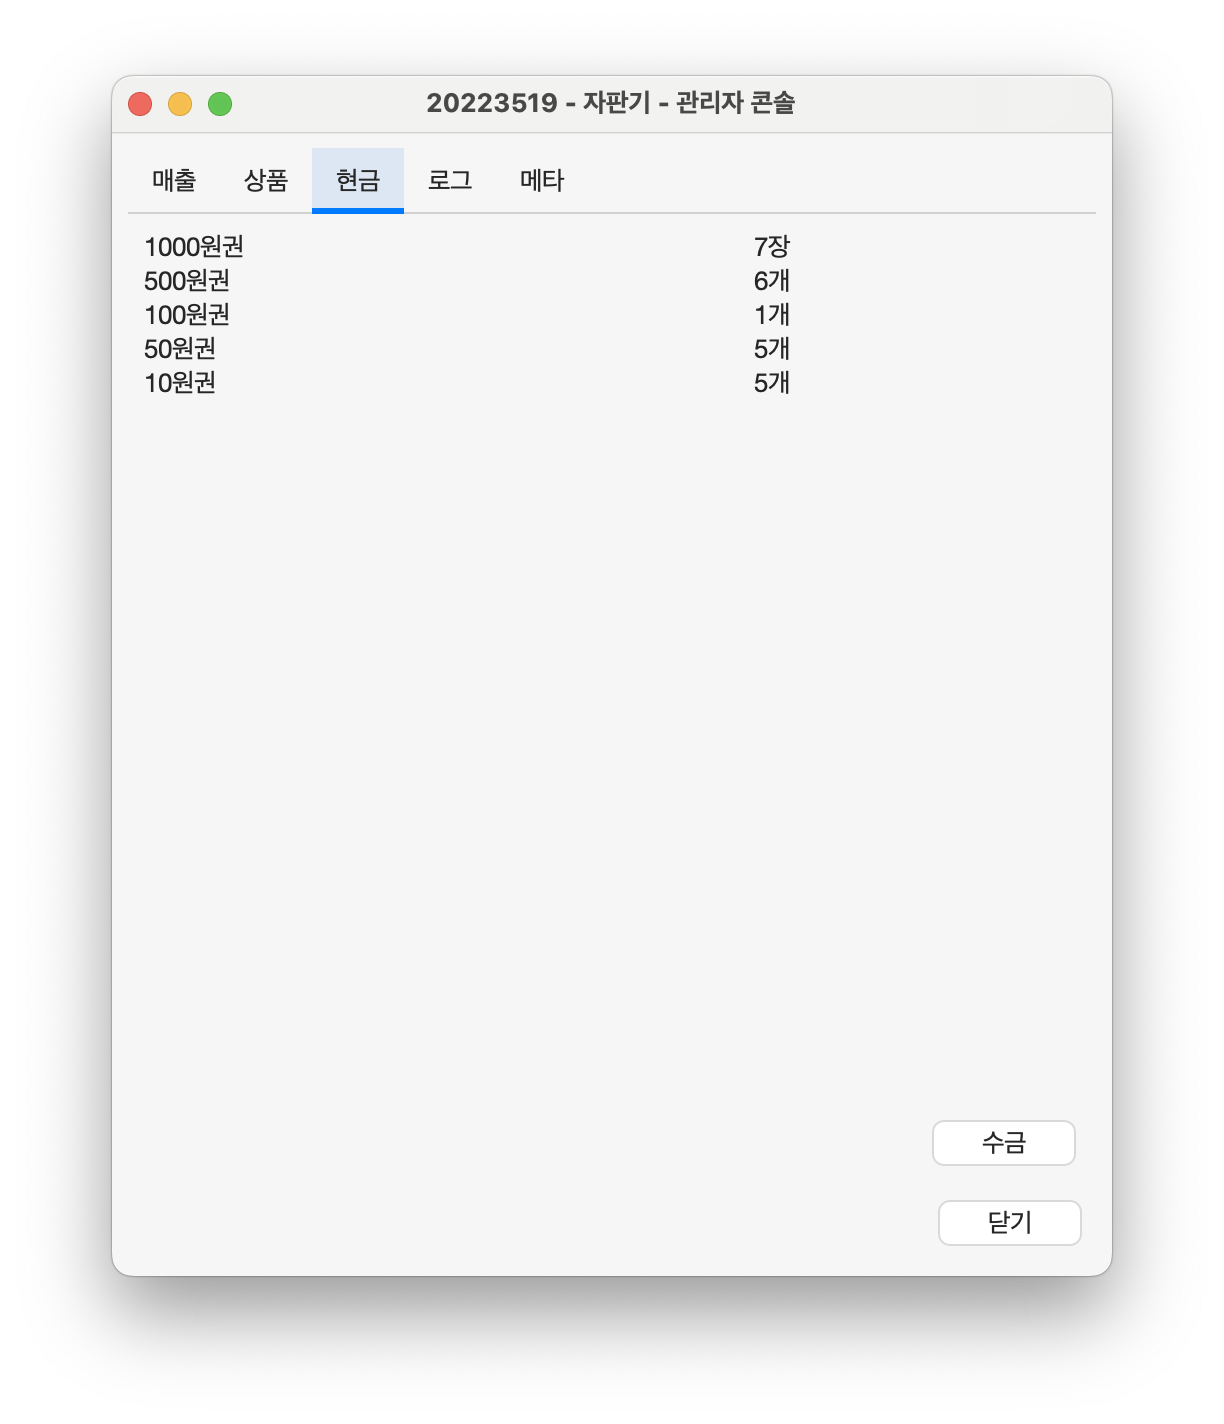
\includegraphics[width=\textwidth]{images/snapshot/admin-cash}
            \caption{관리자 콘솔 현금 수금 탭}
            \label{fig:admin-cash}
        \end{minipage}
        \begin{minipage}{0.5\textwidth}
            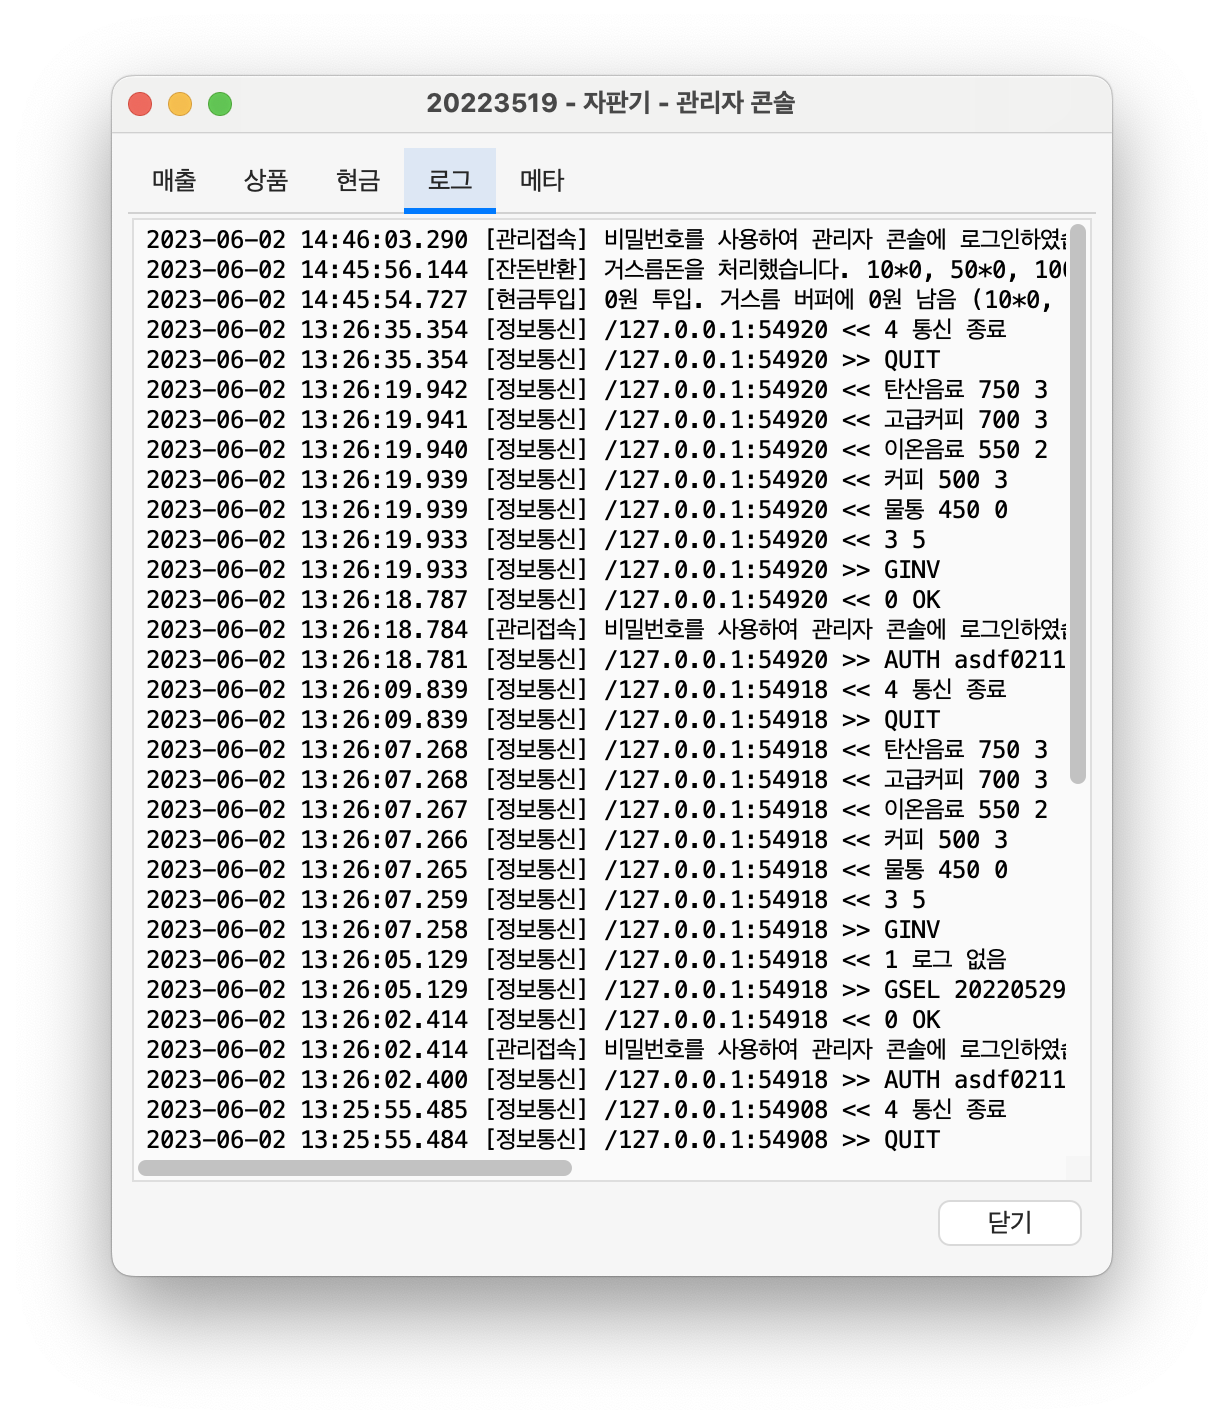
\includegraphics[width=\textwidth]{images/snapshot/admin-log}
            \caption{관리자 콘솔 로그 확인 탭}
            \label{fig:admin-log}
        \end{minipage}%
        \begin{minipage}{0.5\textwidth}
            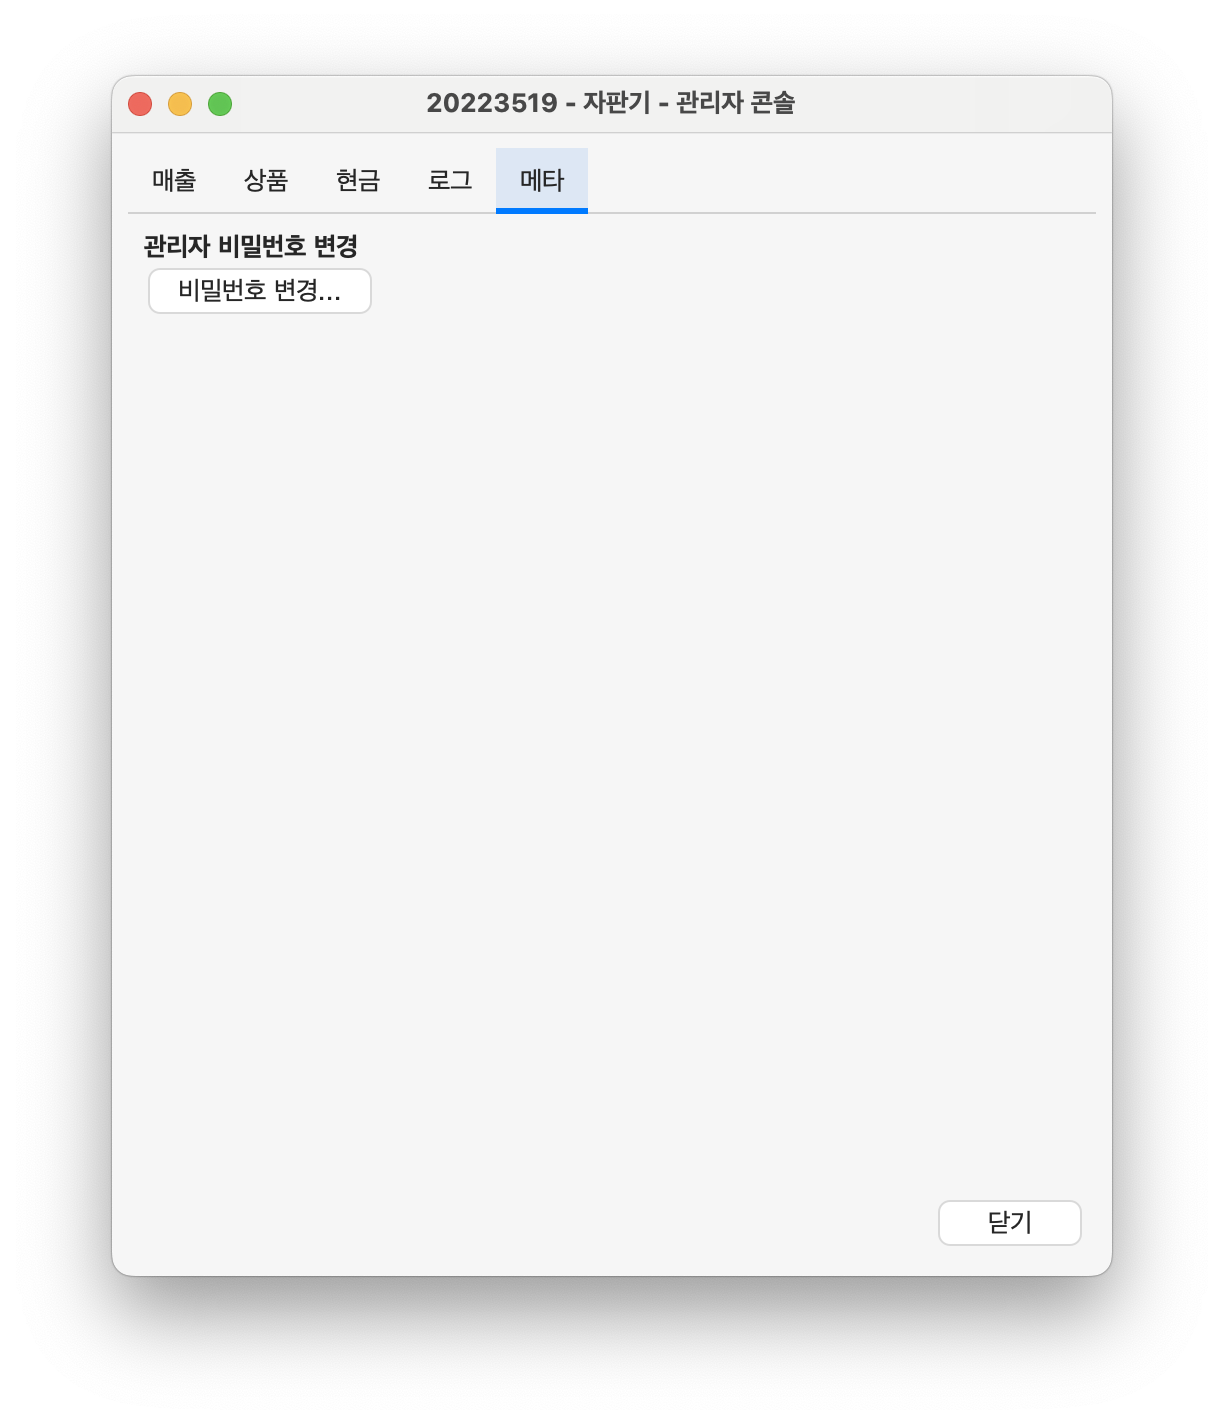
\includegraphics[width=\textwidth]{images/snapshot/admin-meta}
            \caption{관리자 콘솔 메타 탭}
            \label{fig:admin-meta}
        \end{minipage}
    \end{figure}

    \figref{fig:admin-inventory}\는 상품 관리 탭으로,
    자판기에 진열되어있는 상품의 이름과 재고를 확인하고 수정할 수 있다.
    엔트리의 내용을 수정하고 창 오른쪽 아래의 저장 버튼을 누르면 실시간으로 자판기에 반영된다.

    \figref{fig:admin-cash}\는 현금 수금 탭으로,
    현재 자판기에 저장되어있는 현금의 종류별 개수를 확인할 수 있다.
    창 오른쪽 아래에 있는 수금 버튼을 누르면 현금 수금을 할 수 있다.
    이때, 수금을 한 후에도 자판기가 동작해야 하므로 각 화폐권은 5개를 남겨놓도록 수금된다.

    \figref{fig:admin-log}\는 로그 확인 탭으로,
    자판기의 동작 로그를 확인할 수 있다.
    로그는 자판기가 동작할 때마다 자동으로 기록된다.

    \figref{fig:admin-meta}\는 메타 탭으로,
    메타적인 관리를 수행할 수 있다.
    현재는 비밀번호를 바꾸는 기능만 제공되며, 메타 탭에서 ``비밀번호 변경\textellipsis'' 버튼을 누르면
    \figref{fig:password-change}\와 같은 화면이 나타난다.

    \begin{figure}[h]
        \centering
        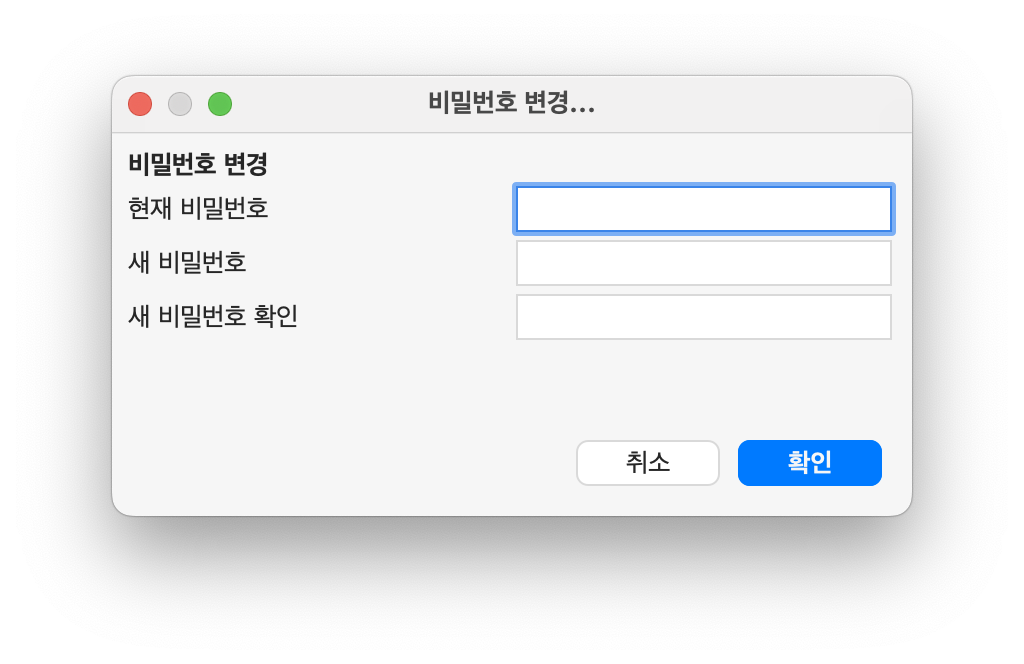
\includegraphics[width=0.5\textwidth]{images/snapshot/password-change}
        \caption{관리자 콘솔 비밀번호 변경 화면}
        \label{fig:password-change}
    \end{figure}

    \subsection{TCP/IP 통신}

    자판기는 기본적으로 \texttt{9832}를 포트 번호로 하는 TCP/IP 서버를 운영한다.
    서버는 클라이언트의 요청을 받아들이고, 요청에 따라 응답을 보낸다.

    \begin{figure}[h]
        \centering
        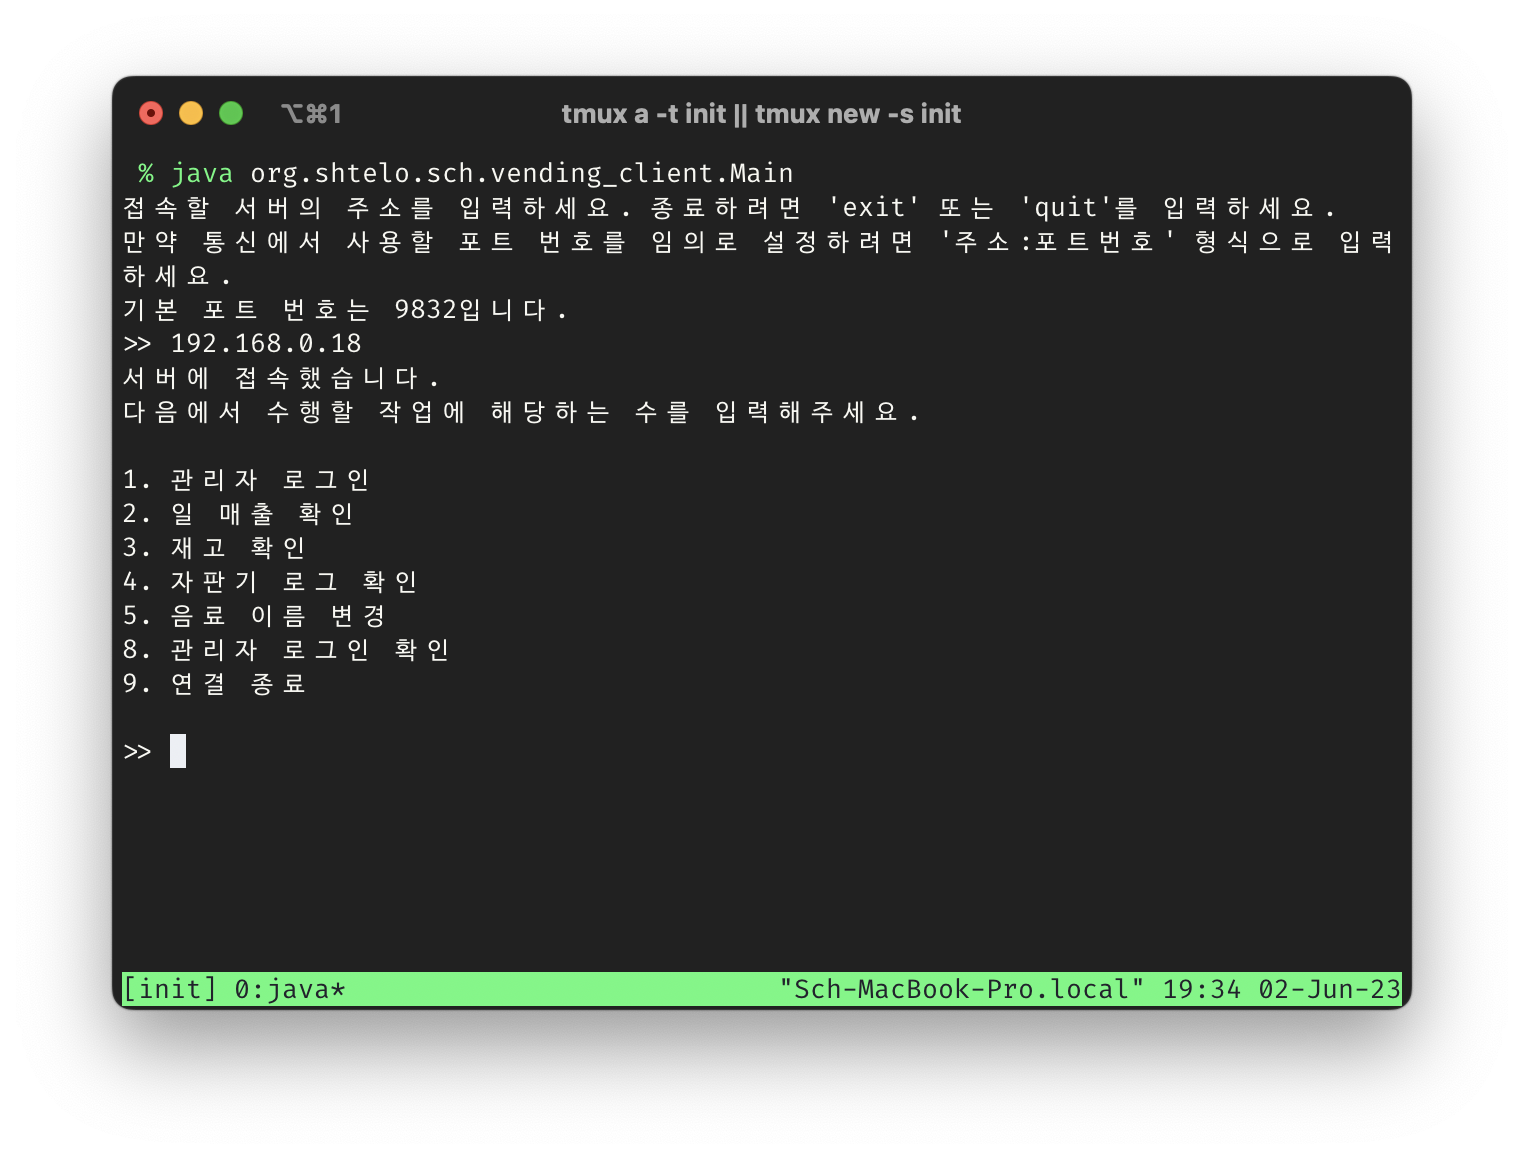
\includegraphics[width=0.5\textwidth]{images/snapshot/client-start}
        \caption{자판기 클라이언트 시작 화면}
        \label{fig:client-start}
    \end{figure}

    \texttt{vending\_client.Main}을 실행하면 자판기가 설치되어있는 컴퓨터의 주소를 입력할 수 있다.
    이곳에 자판기 서버가 설치되어있는 컴퓨터의 주소를 입력하고 엔터를 누르면 자판기에 연결된다.
    \figref{fig:client-start}\는 자판기 클라이언트를 실행하고 주소를 입력해서 자판기에 접속한 모습이다.

    이곳에서는 다음의 7가지 동작을 수행할 수 있다.

    \begin{enumerate}
        \item 관리자 로그인
        \item 일 매출 확인
        \item 재고 확인
        \item 자판기 로그 확인
        \item 음료 이름 변경
        \setcounter{enumi}{7}
        \item 관리자 로그인 확인
        \item 연결 종료
    \end{enumerate}

    연결 종료를 제외한 모든 동작은 관리자 로그인을 선행해야 한다.

    각각의 기능들은 프로토콜을 추상화하여 구현되어 있기 때문에,
    관리자가 직접 서버에 전송될 패킷을 작성할 필요가 없다.

    \section{개발}

    자판기는 \texttt{org.shtelo.sch} 패키지 아래에서 \figref{fig:uml}\과 같은 클래스 구조를 가지고 있다.

    \begin{figure}[h]
        \centering
        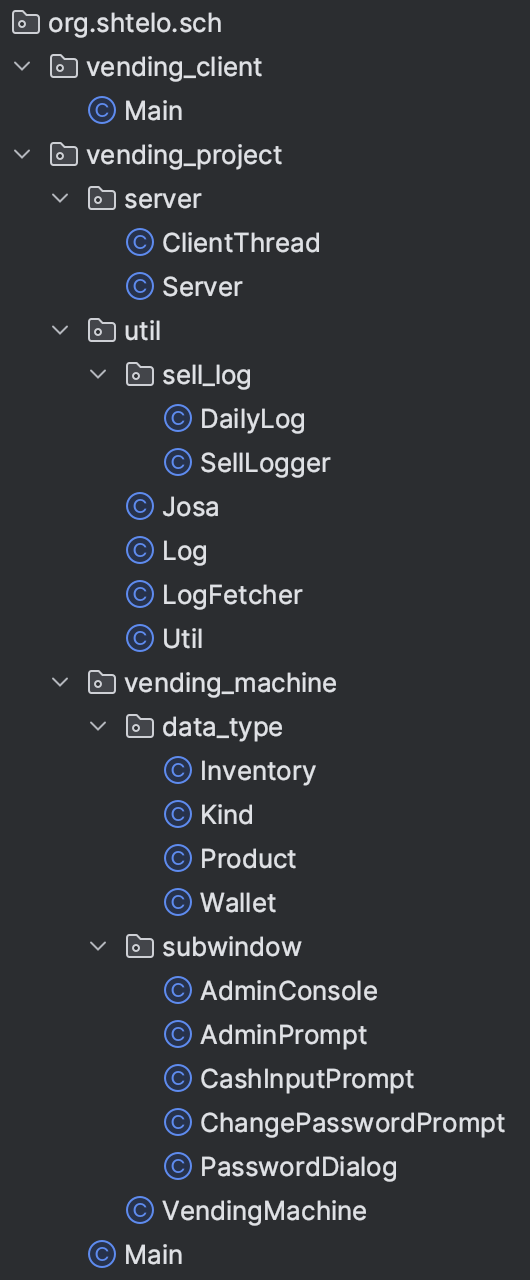
\includegraphics[height=0.5\textheight]{images/class-tree}
        \caption{자판기의 패키지 구조}
        \label{fig:uml}
    \end{figure}

    각각의 클래스에서는 다음과 같은 역할을 수행한다.
    \begin{itemize}
        \item \texttt{vending\_client} -- 자판기 관리자용 클라이언트 패키지
        \item \texttt{vending\_client.Main} --
        자판기 클라이언트의 메인 클래스.
        서버에 있는 자판기 관리자는 이 클래스를 CLI에서 실행하여 원격으로 자판기를 관리한다.
        \item \texttt{vending\_project} -- 자판기 본체를 구현한 패키지
        \item \texttt{vending\_project.server} -- 자판기 본체의 서버 관련 기능을 구현한 패키지
        \item \texttt{vending\_project.server.ClientThread} --
        자판기 서버의 클라이언트 스레드 클래스.
        자판기 서버는 이 클래스의 인스턴스를 생성하여 클라이언트와 통신한다.
        \item \texttt{vending\_project.server.Server} --
        자판기 서버의 메인 클래스.
        자판기 서버는 이 클래스를 실행하여 클라이언트의 접속을 기다린다.
        \item \texttt{vending\_project.util} -- 자판기 본체의 로그, 로그인 등의 유틸리티 기능을 구현한 패키지
        \item \texttt{vending\_project.util.sell\_log} -- 자판기 본체의 판매 기록을 저장하는 패키지
        \item \texttt{vending\_project.util.sell\_log.DailyLog} --
        자판기의 일간 판매 기록을 나타내는 데이터프레임.
        자판기 본체는 이 클래스의 인스턴스를 생성하여 판매 기록을 저장한다.
        \item \texttt{vending\_project.util.sell\_log.SellLogger} --
        자판기의 판매 기록을 저장하는 클래스.
        자판기 본체는 이 클래스의 인스턴스를 생성하여 판매 기록을 저장한다.
        \item \texttt{vending\_project.util.Josa} --
        한글 조사 관련 유틸리티.
        상황에 맞는 조사를 자동으로 선택하여 반환한다.
        \item \texttt{vending\_project.util.Log} --
        자판기 본체의 로그를 출력하는 클래스.
        자판기 본체는 이 클래스의 인스턴스를 생성하여 로그를 기록한다.
        \item \texttt{vending\_project.util.LogFetcher} --
        자판기의 로그를 불러오는 클래스.
        파일에 기록되어있는 파일의 로그를 순서대로 읽어온다.
        \item \texttt{vending\_project.util.Util} --
        기타, 일반적인 유틸리티 기능을 구현한 클래스.
        \item \texttt{vending\_project.vending\_machine} --
        자판기 본체의 자판기 관련 기능을 구현한 패키지
        \item \texttt{vending\_project.vending\_machine.data\_type} --
        자판기에서 사용하는 여러가지 데이터타입을 구현한 패키지
        \item \texttt{vending\_project.vending\_machine.data\_type.Inventory} --
        자판기의 재고를 관리하는 클래스
        \item \texttt{vending\_project.vending\_machine.data\_type.Kind} --
        음료의 종류를 나타내는 클래스.
        이름과 가격 정보가 저장된다.
        \item \texttt{vending\_project.vending\_machine.data\_type.Product} --
        자판기 인벤토리의 각각 항목을 나타내는 클래스.
        음료의 종류와 수량 정보가 저장된다.
        \item \texttt{vending\_project.vending\_machine.data\_type.Wallet} --
        자판기에서 사용할 수 있는 현금 정보를 저장하는 클래스.
        현금의 종류와 수량 정보가 저장된다.
        \item \texttt{vending\_project.vending\_machine.subwindow} --
        자판기 본체의 서브윈도우 관련 기능을 구현한 패키지.
        \item \texttt{vending\_project.vending\_machine.subwindow.AdminConsole} --
        괸리자 콘솔.
        재고 확인, 재고 수정 등 관리자가 사용할 수 있는 기능을 제공한다.
        \item \texttt{vending\_project.vending\_machine.subwindow.AdminPrompt} --
        관리자 콘솔에 접근하기 위한 패스워드를 입력받는 윈도우.
        \item \texttt{vending\_project.vending\_machine.subwindow.CashInputPrompt} --
        현금을 입력받는 윈도우.
        현금의 종류와 수량을 입력받는다.
        \item \texttt{vending\_project.vending\_machine.subwindow.ChangePasswordPrompt} --
        비밀번호 변경 윈도우.
        관리자 비밀번호를 변경할 수 있다.
        \item \texttt{vending\_project.vending\_machine.subwindow.PasswordDialog} --
        비밀번호 초기 설정 윈도우
        \item \texttt{vending\_project.vending\_machine.VendingMachine} --
        자판기 본체 윈도우
        \item \texttt{vending\_project.Main} --
        자판기 본체의 메인 클래스.
        자판기 본체를 실행한다.
    \end{itemize}

    \subsection{3월 14일}\label{subsec:3-14}

    자판기의 개발은 3월 14일에 시작했다.
    이 날 자판기에서 필요로 하는 기능들을 추합했고,
    과제에서 주어지는 요구 사항들을 해결하기 위해서 어떻게 자판기를 구현하면 좋을지 대략적인 구현 방안을 모색했다.
    이때 작성한 요구 사항이~\ref{subsec:requirements}절에 정리되어 있다.

    개발은 Git을 사용하여 버전관리를 진행했다.
    버전관리를 하면 언제 어떤 코드를 작성했는지 추적할 수 있고, 코드를 잃어버려도 복구할 수 있기 때문에
    개발을 할 때는 항상 버전관리를 하는 것이 좋다.

    자판기의 코드는 GitHub에 업로드되어 있고,~\cite{github}에서 확인할 수 있다.
    과제 개발 시점부터 제출 시점까지는 코드 유출 등을 방지하기 위해서 private 레포지토리로 설정해 두었다.
    이 코드는 별 일이 없으면 성적 산출이 모두 끝난 후에 public 레포지토리로 전환할 예정이다.

    3월 14일의 커밋 내역은 다음과 같다.
    \begin{itemize}
        \item Make main file: The initial commit
        \item Design main page
        \item Implement quit button on main window
        \item Set main window minimum size
    \end{itemize}

    일단 \texttt{vending\_machine.VendingMachine} 클래스가 자판기의 메인 화면을 보이도록 GUI를 구현했다.
    이미 몇 년 전에 Java Swing을 활용하여 GUI 프로그램을 만든 경험이 있으므로,
    당시의 기억을 살려서 만들어보았다.

    \texttt{vending\_machine.VendingMachine}에서 자판기의 메인 화면을 구현하고,\\
    \texttt{vending\_machine.Main}에서 해당 메인 화면을 켜는 명령을 내리도록 프로그램을 구성하였다.
    이렇게 구성한 이유는 추후에 서버를 구현할 때,
    서버를 켜는 것과 화면을 켜는 것을 둘 다 \texttt{Main}의 \texttt{main} 함수에서 실행하기 위함이다.

    기본적으로 제공되는 Swing의 테마는 너무 구식이라서, Swing에서 사용할 수 있는 테마를 찾아보았다.
    그 결과 \texttt{FlatLaf}라는 라이브러리를 사용하기로 했다.
    \texttt{FlatLaf}는 \texttt{FlatMacLightLaf}라는 테마를 제공하므로,
    이 테마를 사용하여 자판기의 GUI를 구현하였다.

    3월 14일 개발한 자판기의 초기 화면은 \figref{fig:0314-vending-machine}과 같다.
    \begin{figure}[h]
        \centering
        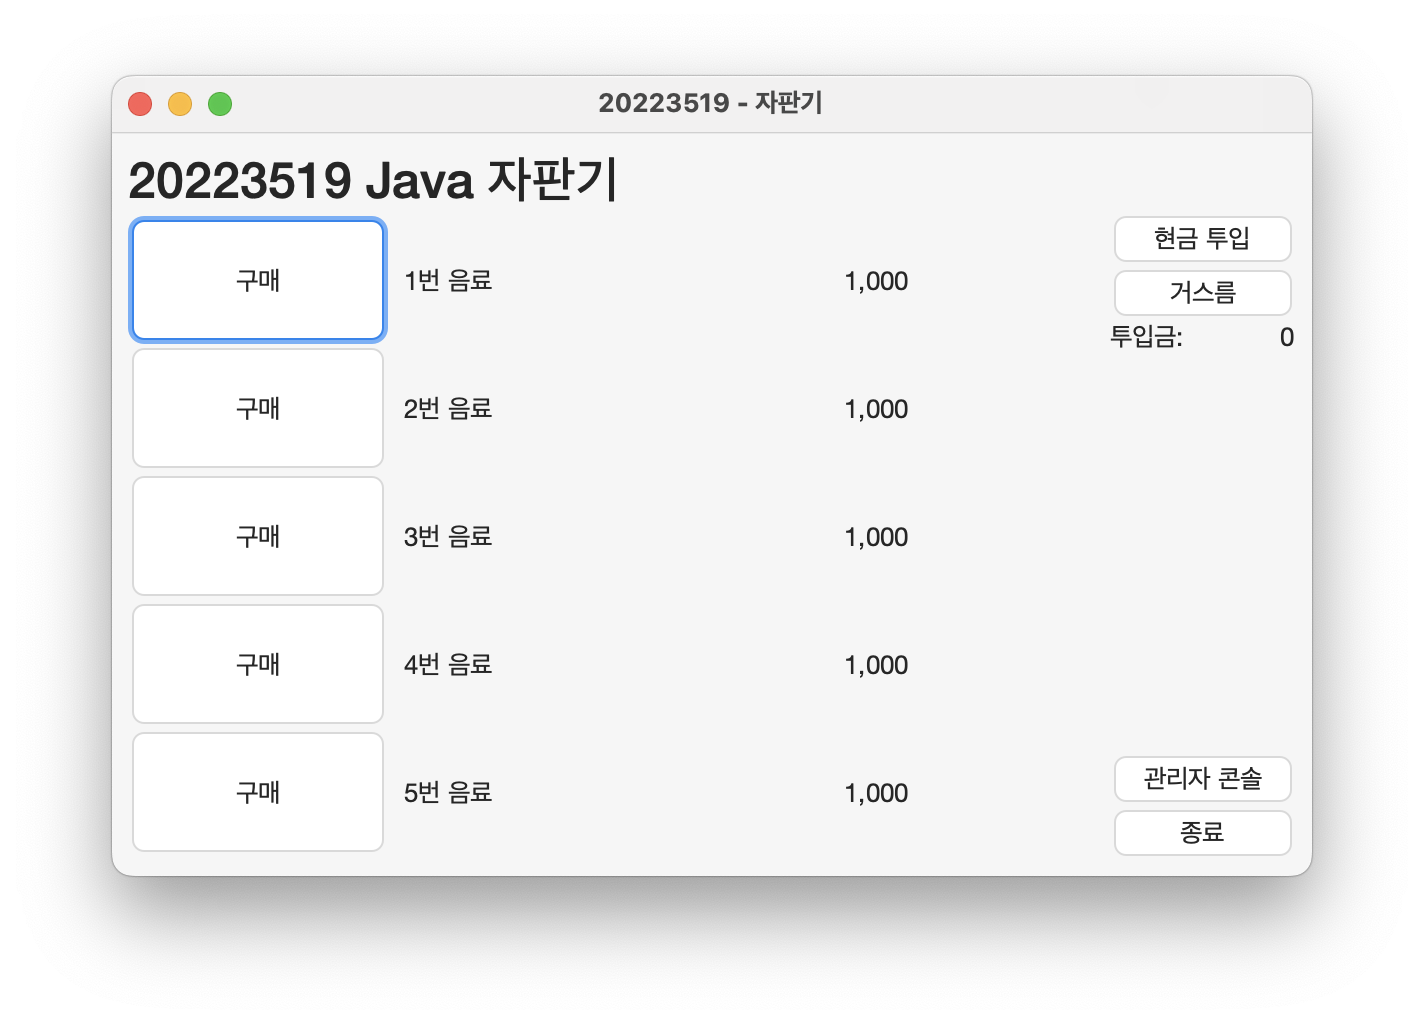
\includegraphics[width=0.5\textwidth]{images/dev-snapshop/0314-vending-machine}
        \caption{3월 14일에 구현한 자판기의 초기 화면}
        \label{fig:0314-vending-machine}
    \end{figure}

    \subsection{3월 15일}

    3월 15일의 커밋 내역은 다음과 같다.
    \begin{itemize}
        \item Implemented vending machine inventory file reading
        \item Implemented creating directory if there's no `res`
        \item Attach comments everywhere
        \item Modify main window minimal size
        \item Separate class into individual files
        \item Make vending machine wallet frame
        \item Implement inserting cash
        \item implement change cash
        \item Cleanup data type class path
        \item Update cash change dialog
        \item Update cash kinds
        \item Update default vending machine inventory
        \item Design meta panel for prevent vertical stretch
        \item Update JavaDoc
        \item Implement product buy
        \item Comment util.Josa
        \item Implement function for updating left product amount
    \end{itemize}

    \begin{figure}[h]
        \centering
        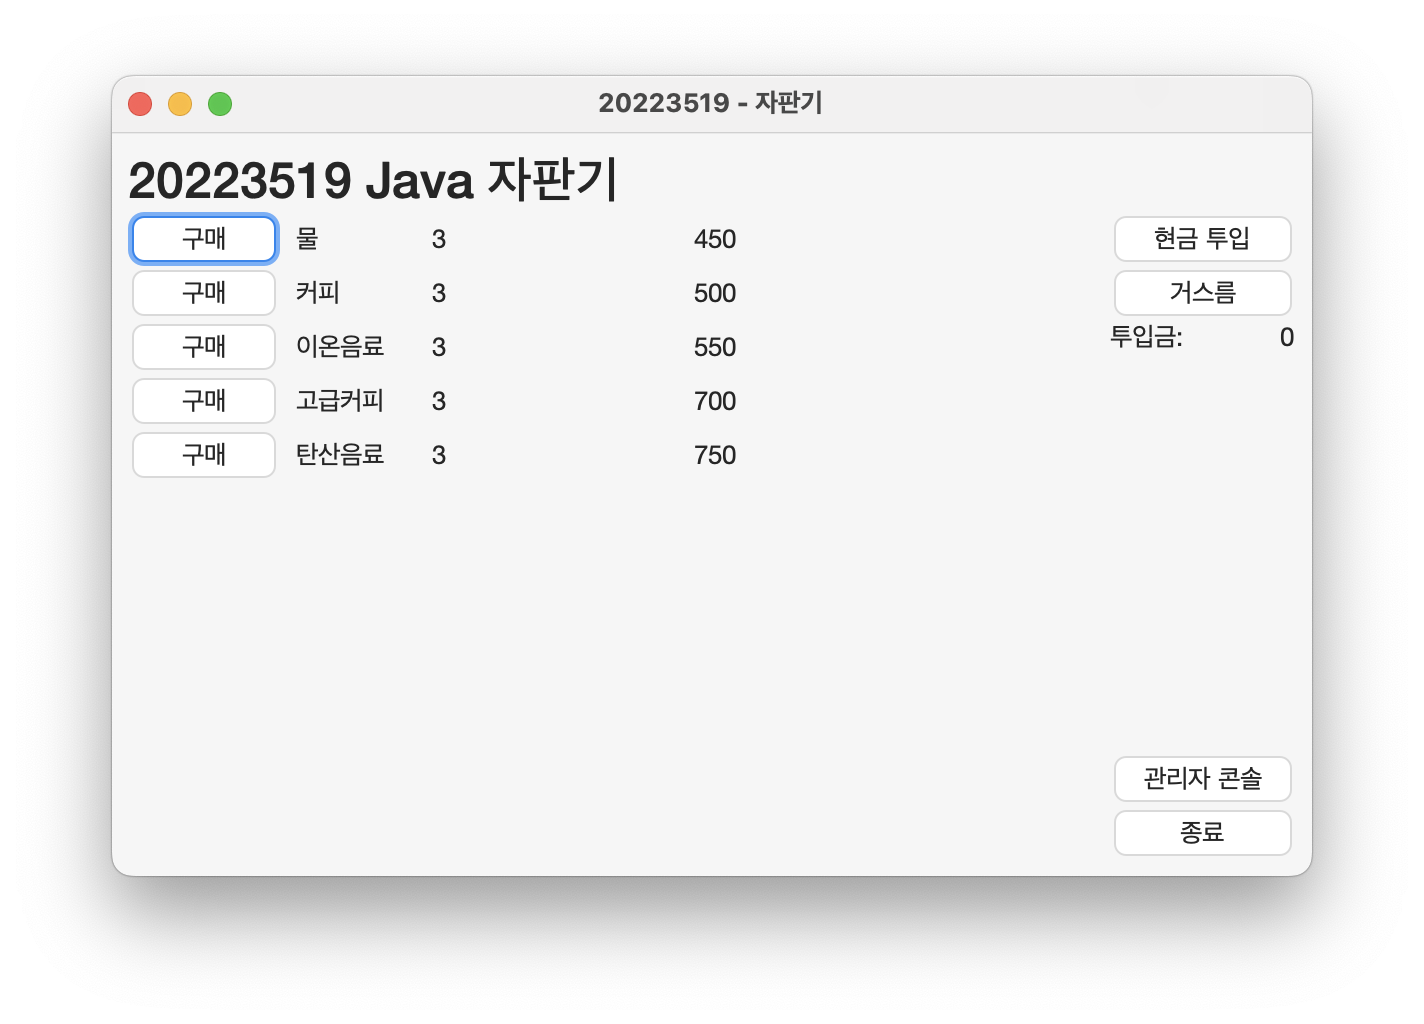
\includegraphics[width=0.5\textwidth]{images/dev-snapshop/0315-vending-machine}
        \caption{3월 15일에 구현한 자판기의 초기 화면}
    \end{figure}

    자판기의 인벤토리를 파일에 입출력하는 부분을 구현했다.
    문제에서 주어진 기본값을 코드에서 제작하도록 하고,
    만약 이미 저장되어있는 파일이 없는 경우에, 프로그램에서 만든 기본값을 파일에 저장하여
    그 파일을 사용하도록 만들었다.

    서브윈도우를 만들어 현금 입력 용량을 사용자가 입력할 수 있도록 했다.
    그리고 자판기에서 사용할 수 있는 현금 정보를 저장하는 \texttt{Wallet} 클래스를 구현했다.
    \texttt{Wallet} 클래스는 10원권부터 1,000원권까지를 각각 몇 개씩 가지고 있는지 변수로 저장하여 현금 정보를 관리한다.
    이때, 현금 정보 역시 자판기를 껐다가 켜도 그대로 사용할 수 있도록 파일 입출력으로 저장하도록 하였다.
    현금 입력 서브윈도우는 \figref{fig:0315-cash-input-prompt}\과 같다.
    \begin{figure}[h]
        \centering
        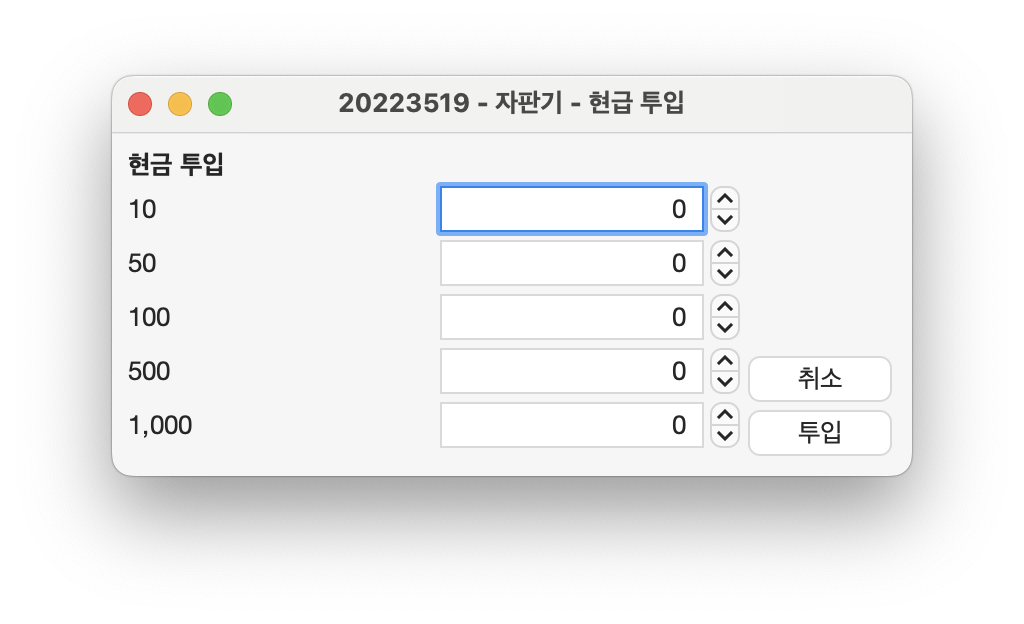
\includegraphics[width=0.5\textwidth]{images/dev-snapshop/0315-cash-input-prompt}
        \caption{3월 15일에 구현한 현금 입력 서브윈도우}
        \label{fig:0315-cash-input-prompt}
    \end{figure}

    원래는 10원권부터 10,000원권까지를 자판기에서 처리할 수 있도록 할 예정이었으나,
    문제 조건 상 한 번에 5,000원 이상, 지폐로는 3,000원 이상을 투입할 수 없도록 만들라고 했기 때문에
    1,000원권까지 관리하도록 구현했다.

    \figref{fig:0315-change-dialog}\은 거스름돈을 처리한 결과를 알려주는 다이얼로그이다.
    \begin{figure}[h]
        \centering
        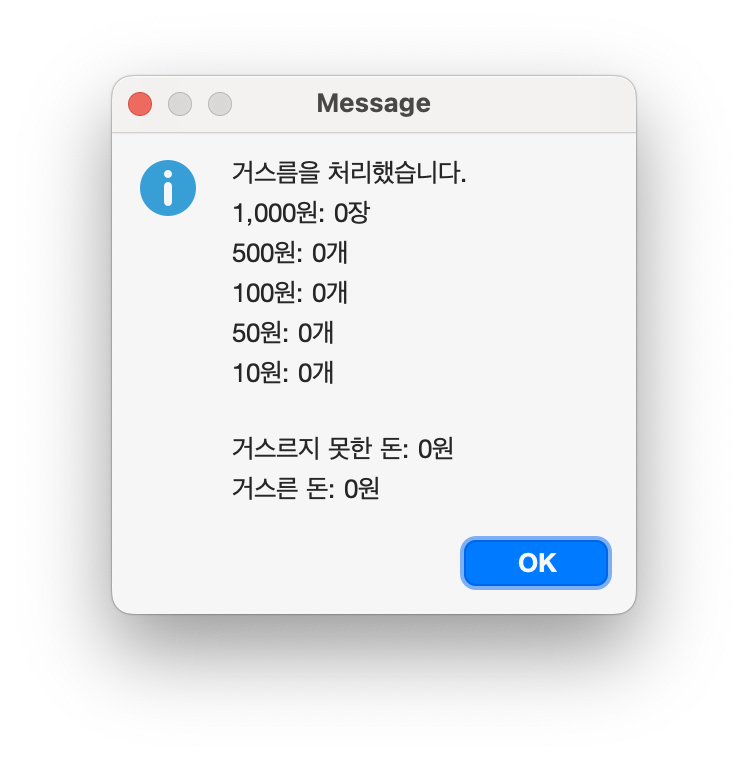
\includegraphics[width=0.5\textwidth]{images/dev-snapshop/0315-change-dialog}
        \caption{3월 15일에 구현한 거스름돈 다이얼로그}
        \label{fig:0315-change-dialog}
    \end{figure}

    파일에 자료를 저장할 때에는 개발자가 프로그램을 켜지 않을 때에도 수정하기 편하도록 JSON 형식으로 저장하도록 했다.
    Java에서 기본적으로 JSON 형식 파일 입출력을 지원하지 않기 때문에, \texttt{Gson}이라고 하는 외부 라이브러리를 사용하여
    JSON 형식으로 파일입출력을 수행했다.

    GUI를 코드에서 구현하고 있으므로 화면을 디자인하는 데에 어려움을 겪었다.
    HTML과 완전히 다른 방식으로 화면이 구성되므로 Java Swing을 사용해서 원하는 레이아웃을 구현하는 것이 어려웠다.

    음료를 구매한 후에는 ``(음료 이름)을(를) 1개 구매했습니다.''라고 하는 메시지가 포함된
    다이얼로그를 화면에 표시하도록 했는데, 이때 음료 이름에 따라서 목적격 조사 `을', `를'을 올바르게 자동으로 선택하게 하도록 하기 위해서
    \texttt{Josa} 유틸리티를 구현했다.

    \subsection{3월 16일}

    3월 16일의 커밋 내역은 다음과 같다.
    \begin{itemize}
        \item Change CashInputPrompt to JDialog shown
        \item Update CashInputPrompt minimum size
        \item Remove cash insert dialog always on top
        \item Implemented Inventory, wallet auto-save
        \item Set cash insert limit
        \item Change package name
        \item Remove un-used command
        \item Make admin prompt frame
        \item Implement press enter key to submit on dialogs
    \end{itemize}

    자판기의 현금 투입 다이얼로그를 \texttt{JDialog}로 구현했다.
    원래는 \texttt{JFrame}으로 단지 새로운 창을 띄우는 것으로 해결하려고 했는데,
    \texttt{JFrame}으로 구현하면 자판기의 메인 화면 뒤로 가려져서 사용자가 현금 투입 다이얼로그를 볼 수 없었다.
    \texttt{JDialog}로 구현하면 자판기의 메인 화면 뒤로 가려지지 않고, 사용자가 현금 투입 다이얼로그를 볼 수 있도록 할 수 있었다.

    그리고 관리자 콘솔 로그인을 구현하기 위해 비밀번호 입력 다이얼로그를 \figref{fig:0316-password-dialog}\와 같이 구현했다.
    \texttt{JDialog}로 구현했으며, 비밀번호를 입력하고 엔터 키를 누르면 비밀번호를 확인하도록 했다.
    \begin{figure}[h]
        \centering
        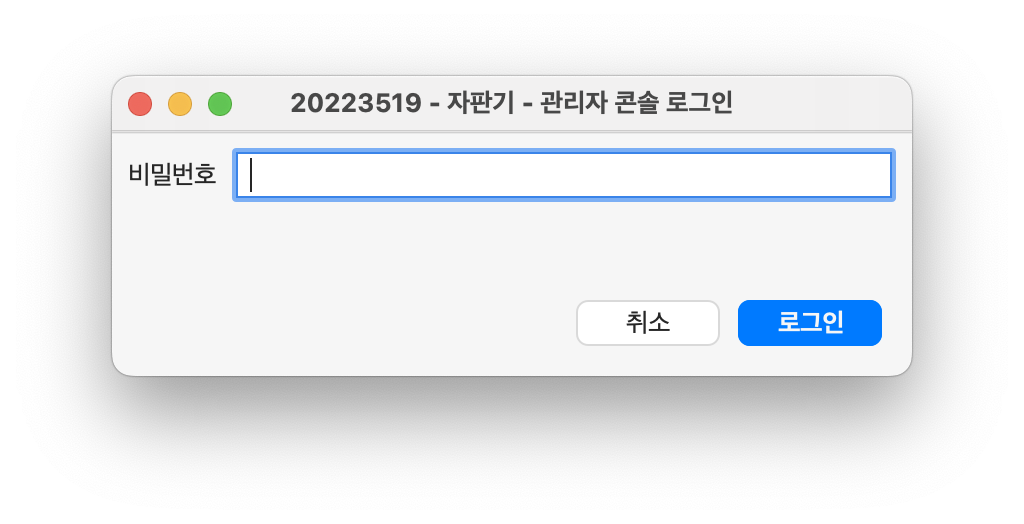
\includegraphics[width=0.5\textwidth]{images/dev-snapshop/0316-password-dialog}
        \caption{3월 16일에 구현한 관리자 콘솔 로그인 다이얼로그}
        \label{fig:0316-password-dialog}
    \end{figure}

    \subsection{3월 20일}

    3월 20일의 커밋 내역은 다음과 같다.
    \begin{itemize}
        \item Implement password creating dialog
        \item Implement AdminPrompt login
        \item Change PasswordDialog handling method
    \end{itemize}

    관리자 콘솔 로그인 다이얼로그를 구현했다.
    만약 비밀번호가 이미 지정되어있지 않다면 \figref{fig:0320-password-not-set}\와 같이
    비밀번호를 설정하는 창을 띄우도록 했다.
    \begin{figure}[h]
        \centering
        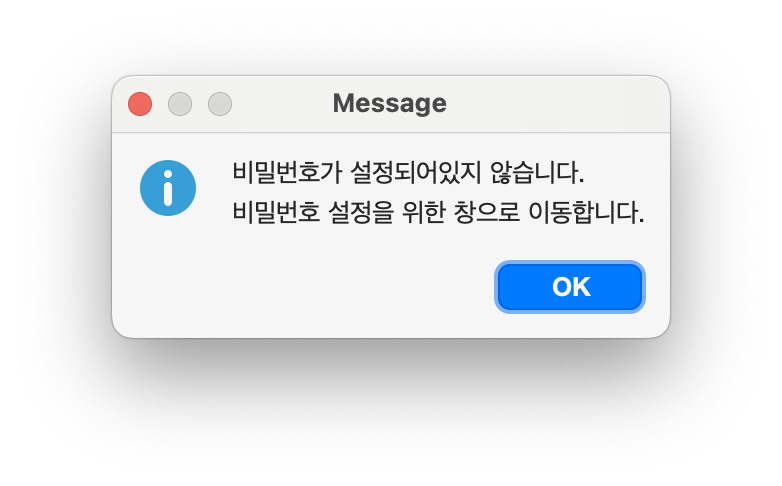
\includegraphics[width=0.5\textwidth]{images/dev-snapshop/0320-password-not-set}
        \caption{3월 20일에 구현한 비밀번호 미설정 다이얼로그}
        \label{fig:0320-password-not-set}
    \end{figure}

    이때, 과제에서 제시된 대로 8자리 이상, 대소문자 포함, 특수문자와 숫자가 포함되도록
    비밀번호를 설정하도록 했다.
    만약 그렇게 비밀번호를 입력하지 않았다면 비밀번호 설정을 확인하지 못하도록 했고,
    재확인 비밀번호를 입력하여 비밀번호를 확인하도록 했다.
    \begin{figure}[h]
        \centering
        \begin{minipage}{.5\textwidth}
            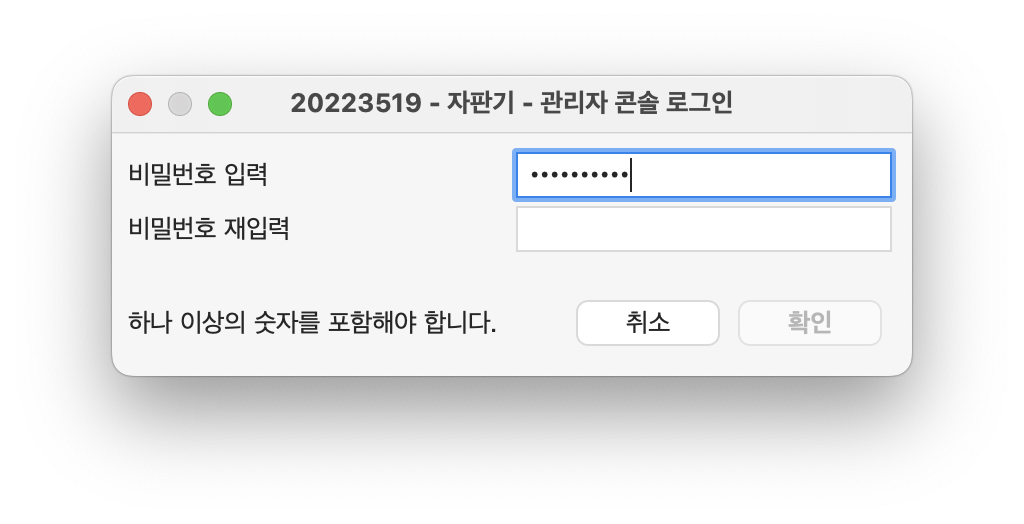
\includegraphics[width=\textwidth]{images/dev-snapshop/0320-password-dialog-1}
            \caption{3월 20일에 구현한 비밀번호 다이얼로그 조건 불만족}
            \label{fig:0320-password-dialog-1}
        \end{minipage}%
        \begin{minipage}{.5\textwidth}
            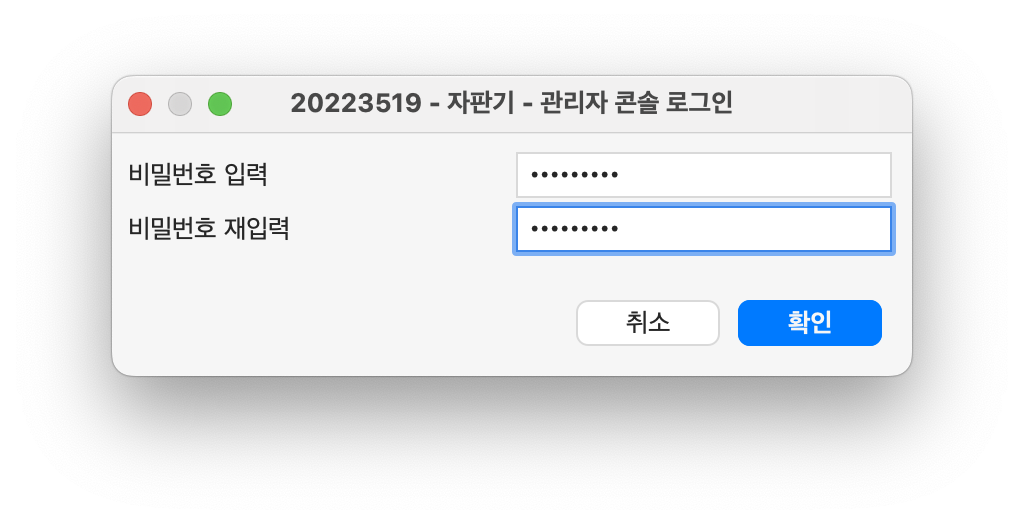
\includegraphics[width=\textwidth]{images/dev-snapshop/0320-password-dialog-2}
            \caption{3월 20일에 구현한 비밀번호 다이얼로그 조건 만족}
            \label{fig:0320-password-dialog-2}
        \end{minipage}
    \end{figure}

    \subsection{3월 21일}

    3월 21일의 커밋 내역은 다음과 같다.
    \begin{itemize}
        \item Resize new password dialog
        \item Make frame for admin console
        \item Make AdminConsole frame
        \item Make admin console inventory panel
        \item Implement password encryption
        \item Comment util functions
        \item Implement logging
        \item Add loggers to events
    \end{itemize}

    관리자 콘솔에서 확인할 로그를 작성하기 시작했다.
    발생하는 여러가지 로그들을 시간과 세션에 따라 따로 저장하여 한 파일의 크기가 너무 커져 읽는 데에 시간이 오래 걸리는 것을 방지했다.
    로그는 날짜마다, 세션마다 각각 다른 폴더와 파일에 행별로 저장된다.

    관리자 콘솔 로그인을 위한 비밀번호를 암호화하여 저장했다.
    비밀번호를 암호화할 때에는 \texttt{SHA-256} 해시 함수를 사용했고,
    레인보우 테이블 공격을 방지하기 위해 비밀번호에 솔트를 추가했다.
    물론 솔트가 언제나 같은 값이므로 방지가 탁월한 효과를 가지지는 않지만,
    일반인이 쉽게 비밀번호를 알아내지 못하도록 하는 데에는 충분하다.

    관리자 콘솔 구현을 위한 프레임을 구현했다.
    관리자 콘솔은 여러가지 작업을 수행할 수 있도록 만들어야 하기 때문에
    \figref{fig:0321-admin-console}\와 같이 탭으로 창을 나누어 사용할 수 있도록 했다.
    \begin{figure}[h]
        \centering
        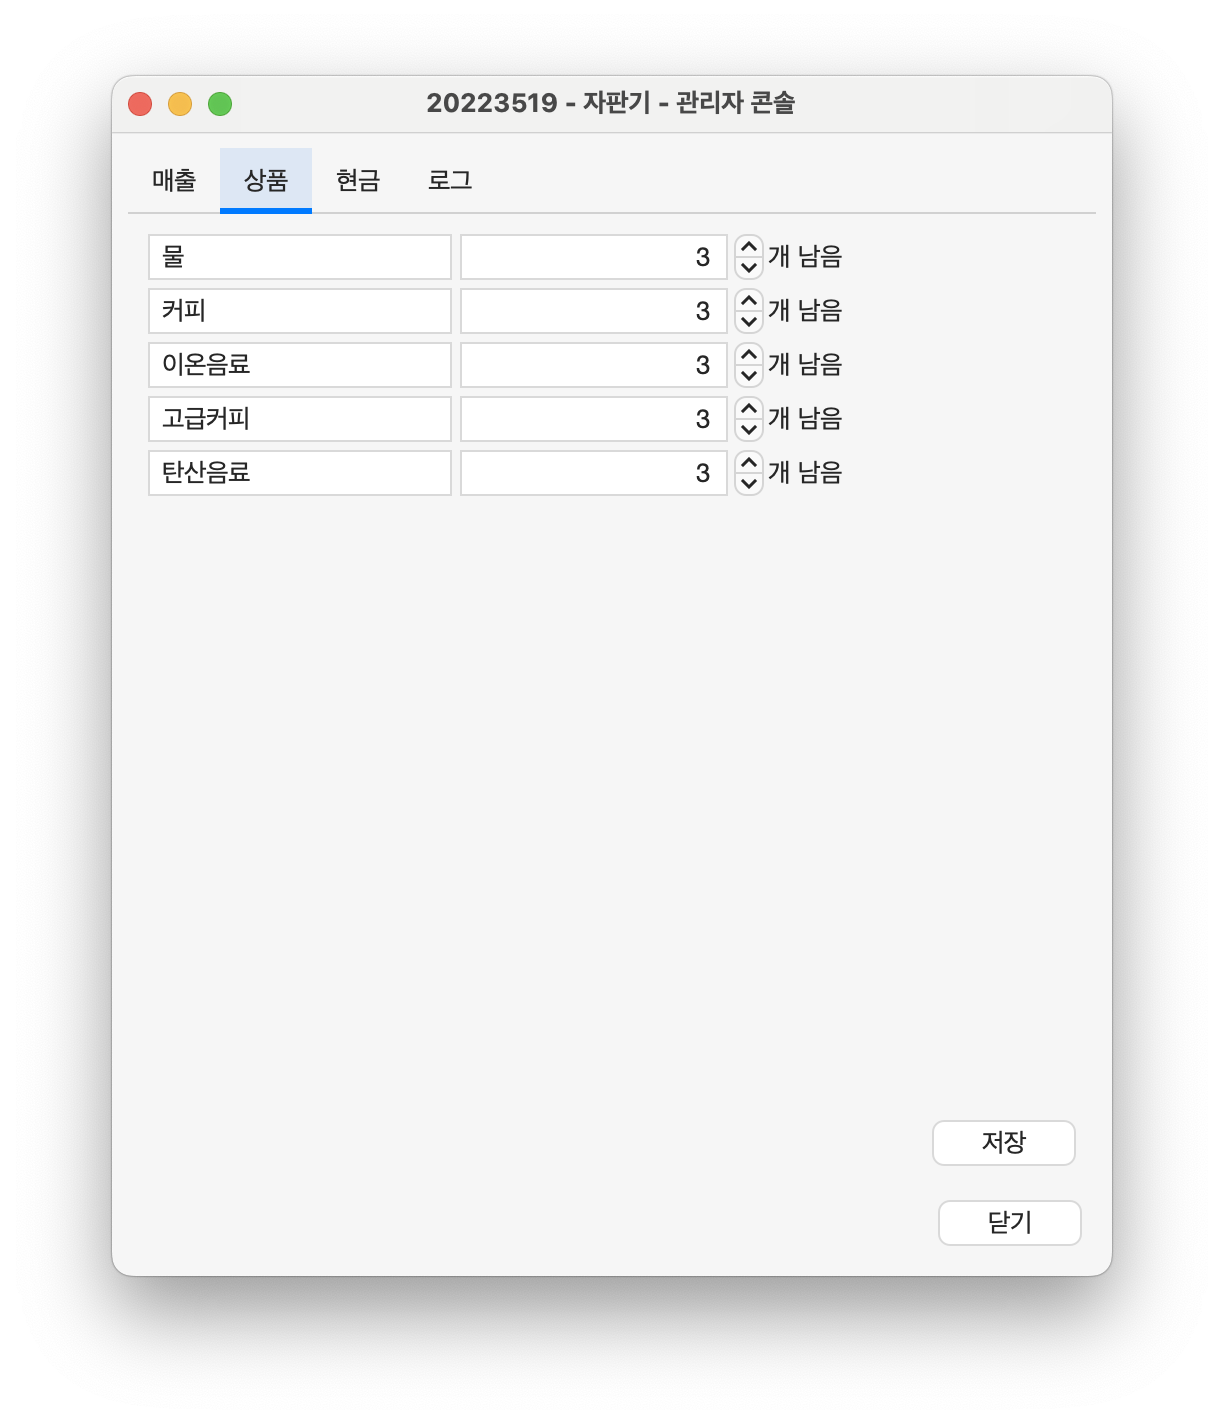
\includegraphics[width=0.5\textwidth]{images/dev-snapshop/0321-admin-console}
        \caption{3월 21일에 구현한 관리자 콘솔 프레임}
        \label{fig:0321-admin-console}
    \end{figure}

    \subsection{3월 22일}

    3월 22일의 커밋 내역은 다음과 같다.
    \begin{itemize}
        \item Implement vacate password on wrong trial
        \item Implement left product count set and log
        \item Implement log on cash change
        \item Implement log on admin login and logout
        \item Implement log login fail
        \item Make frame for meta panel on admin console
        \item Change loggin method
    \end{itemize}

    3월 22일에는 여러가지 상황에서 로그를 작성하도록 업데이트했다.
    이렇게 작성된 로그는 관리자 패널에서 확인할 수 있게 될 것이다.

    이때 새로운 브랜치 \texttt{gui-editor}를 제시했다.

    \begin{itemize}
        \item Use form to build VendingMachine page
    \end{itemize}

    이 브랜치는 관리자 콘솔의 GUI를 Form을 사용하여 구현하는 브랜치이다.
    하지만 담당 교수님께 문의한 결과 웬만하면 form을 사용하지 말라는 답변을 받았기에
    이 브랜치는 더 이상 사용하지 않기로 했다.
    \figref{fig:0322-vending-machine}\은 이 브랜치를 사용하여 구현한 자판기 프레임이다.
    \begin{figure}[h]
        \centering
        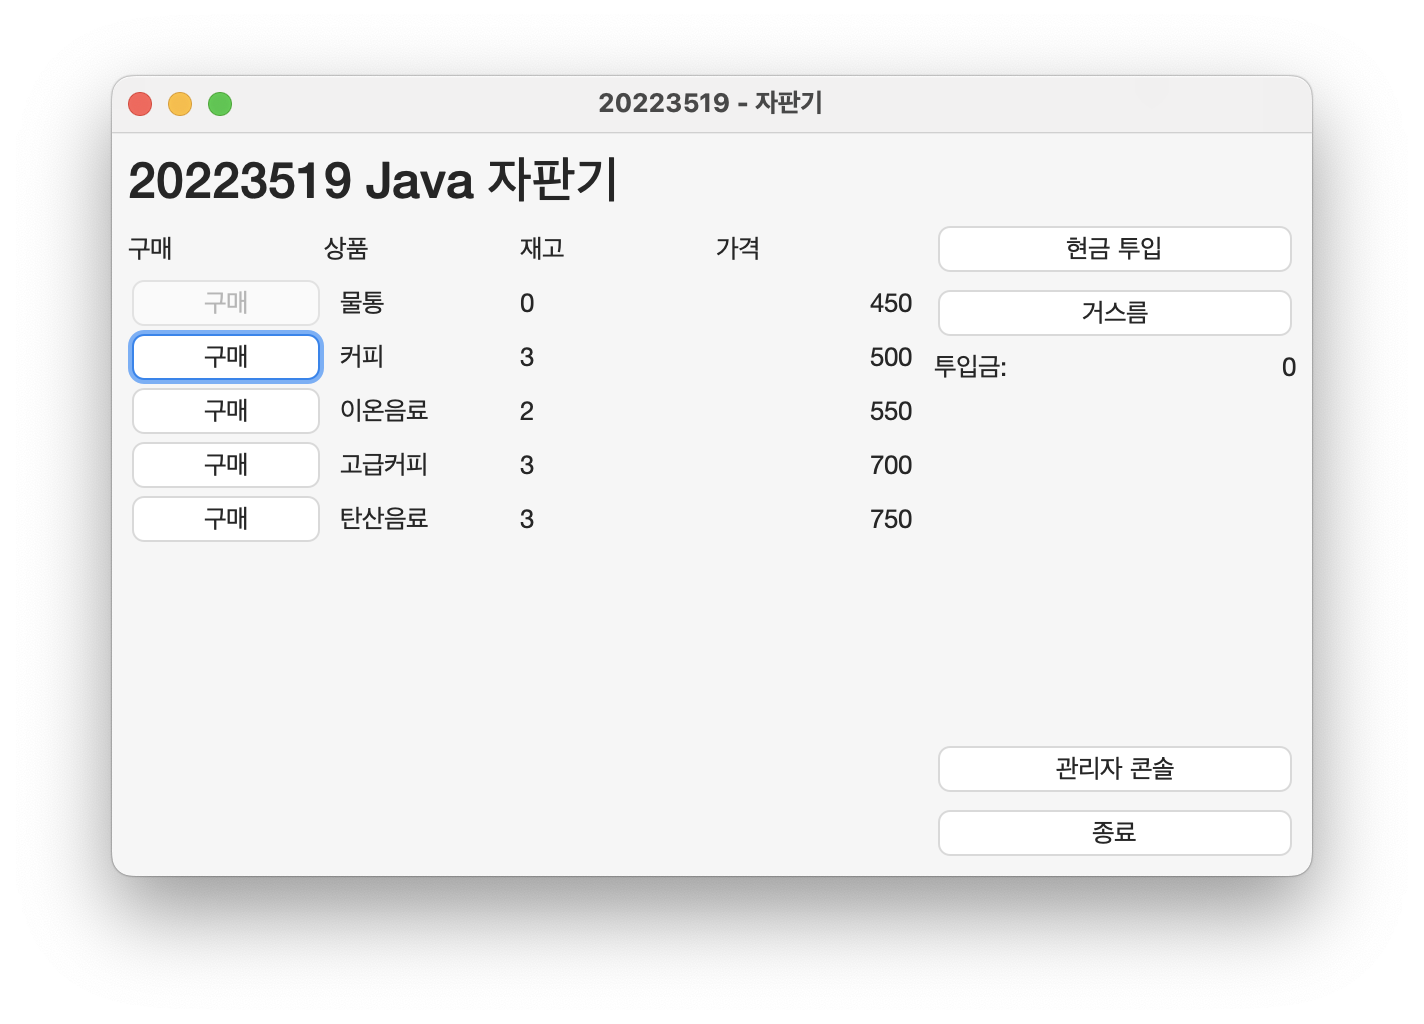
\includegraphics[width=0.5\textwidth]{images/dev-snapshop/0322-vending-machine}
        \caption{3월 22일에 Form으로 구현한 자판기 프레임}
        \label{fig:0322-vending-machine}
    \end{figure}

    \subsection{4월 5--22일}

    4월 5일과 4월 22일의 커밋 내역은 다음과 같다.
    \begin{itemize}
        \item Implement change password
        \item Implement product name change
        \item Make frame of taking cashes on AdminConsole
        \item Implement cash taking
        \item Save cash buffer for the next machine session
        \item Rearrange code
    \end{itemize}

    관리자가 원하는 경우 비밀번호를 변경할 수 있도록 \figref{fig:0405-password-change}\와 같이 비밀번호 변경 화면을 구현했다.
    \begin{figure}[h]
        \centering
        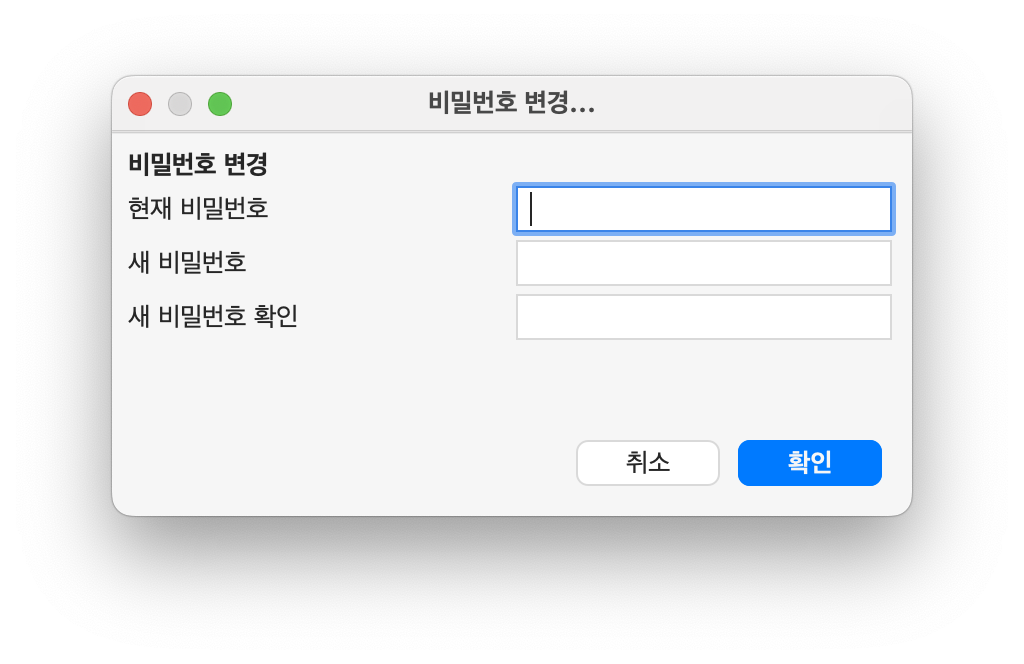
\includegraphics[width=0.5\textwidth]{images/dev-snapshop/0405-password-change}
        \caption{4월 5일에 구현한 비밀번호 변경 화면}
        \label{fig:0405-password-change}
    \end{figure}

    그리고 관리자가 원하는 경우 현금을 수금할 수 있도록 \figref{fig:0405-cash-take}\와 같이 현금 수금 현황 확인표와 수금 버튼을 구현했다.
    이 경우 과제에서 제시된 조건과 같이 5개 이상 화폐권이 남도록 수금 개수를 제한했다.
    \begin{figure}[h]
        \centering
        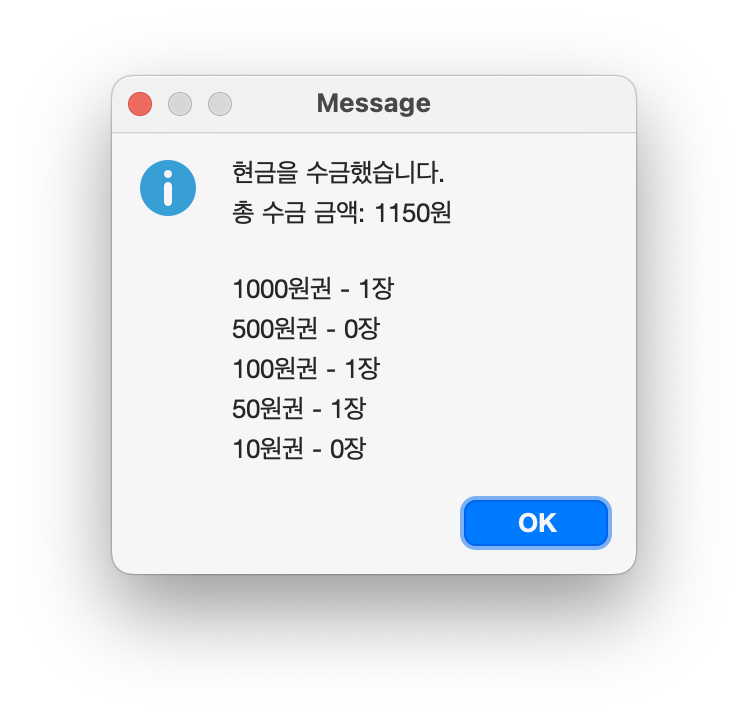
\includegraphics[width=0.5\textwidth]{images/dev-snapshop/0405-cash-take}
        \caption{4월 5일에 구현한 현금 수금 화면}
        \label{fig:0405-cash-take}
    \end{figure}

    \subsection{4월 27일--5월 21일}

    4월 27일과 5월 21일의 커밋 내역은 다음과 같다.
    \begin{itemize}
        \item Create frame of LogFetcher
        \item Implemented Log Viewer
        \item Handle logger exception
        \item Catch exception to not enough logs
        \item Handle LogFetcher exception
    \end{itemize}

    이 작업일들에는 관리자 콘솔에서 로그를 확인할 수 있도록 했다.
    원래는 로그 확인 일자와 개수 등을 직접 설정하여 로그를 확인할 수 있도록 하는 것이 목표였으나,
    로그를 작성한 방법이 이것을 하기가 번거로워 일단 최신 로그 순으로 몇 개만 확인할 수 있도록 로그 확인 화면을
    \figref{fig:0427-log-console}\와 같이 구현했다.
    \begin{figure}[h]
        \centering
        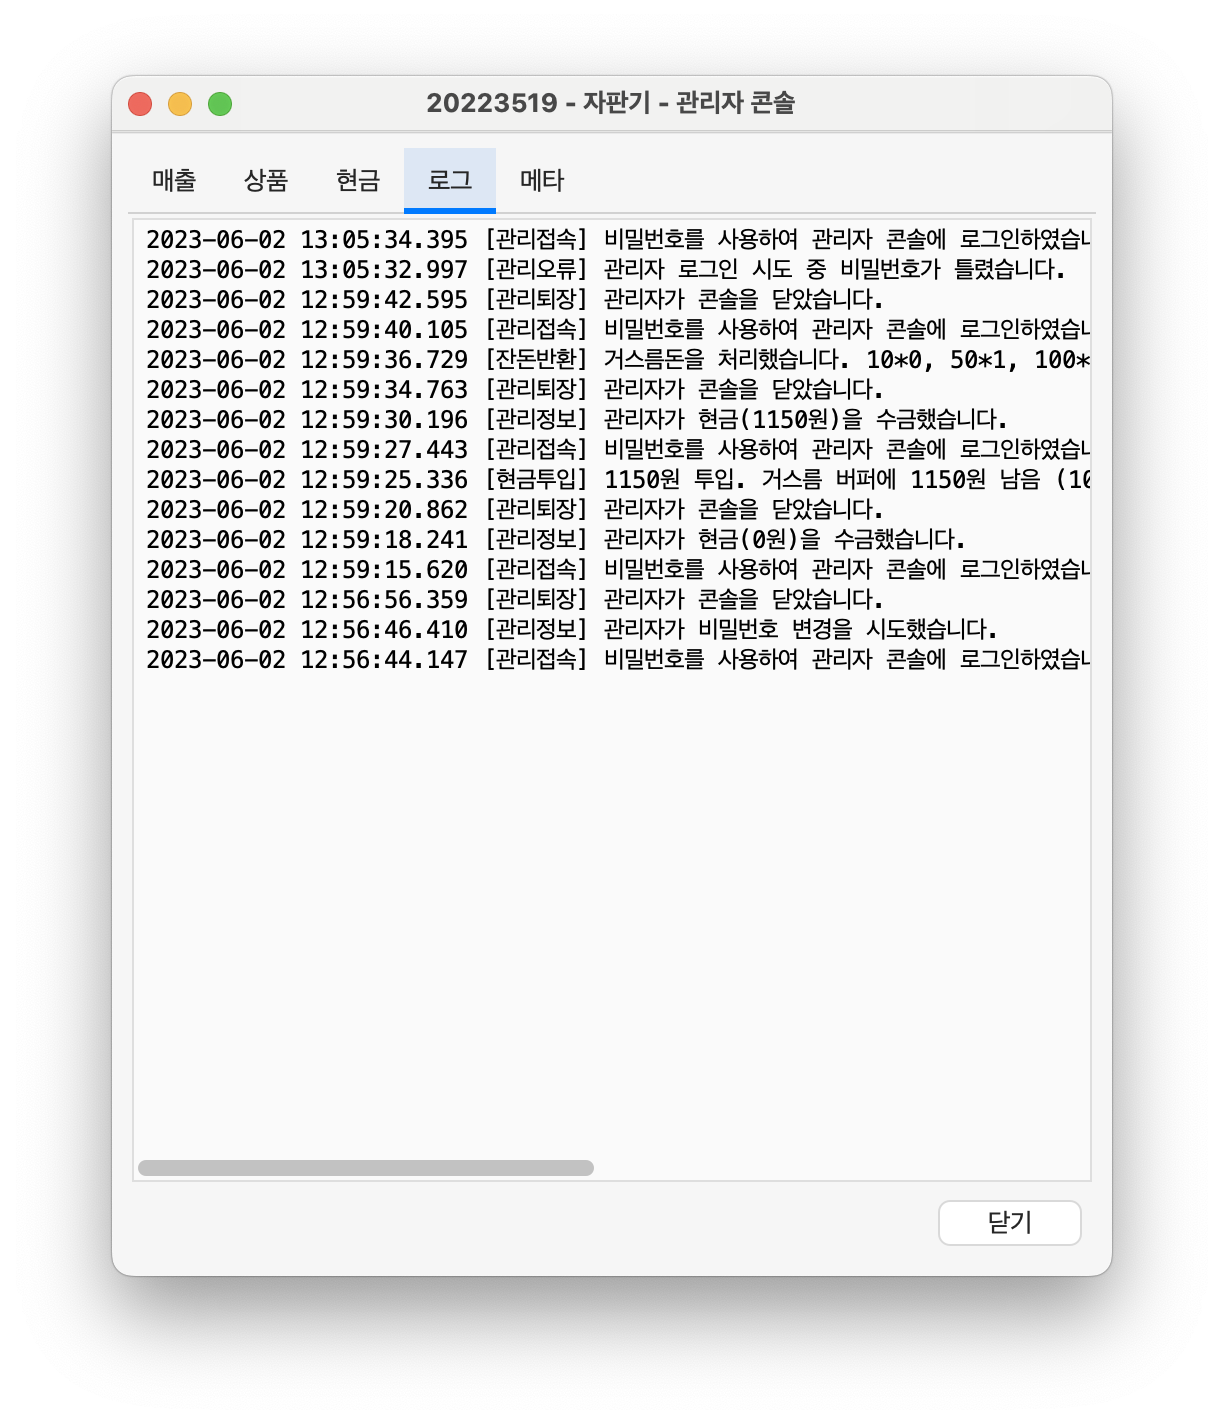
\includegraphics[width=0.8\textwidth]{images/dev-snapshop/0427-log-console}
        \caption{4월 27일에 구현한 로그 확인 화면}
        \label{fig:0427-log-console}
    \end{figure}

    \subsection{5월 24일}

    5월 24일의 커밋 내역은 다음과 같다.
    \begin{itemize}
        \item Add daily logger
        \item implement display logger on AdminConsole
        \item implement sold out logging
    \end{itemize}

    5월 24일에는 일별 매출을 기록하여 관리자 콘솔에서 확인할 수 있도록 했다.
    일별 매출은 판매되는 음료의 이름이 같으면 같은 것으로 취급하여 매출을 계산한다.
    일별 매출 확인 화면은 \figref{fig:0524-daily-log}\와 같다.
    \begin{figure}[h]
        \centering
        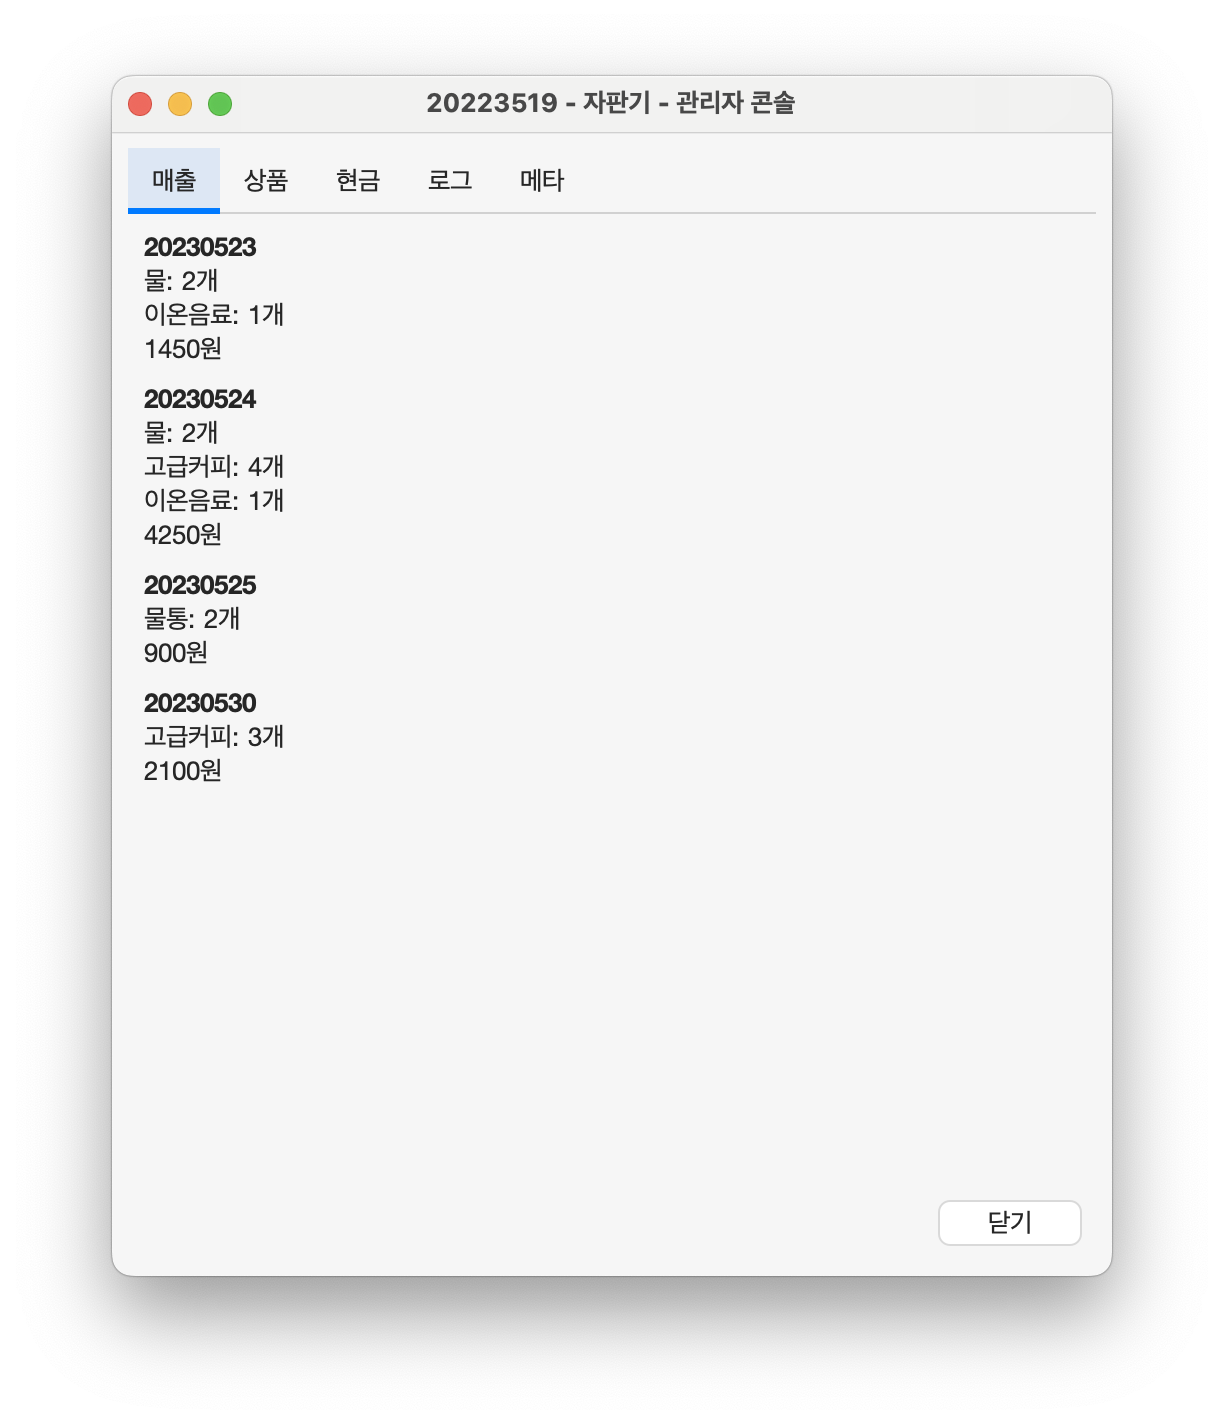
\includegraphics[width=0.8\textwidth]{images/dev-snapshop/0524-daily-log}
        \caption{5월 24일에 구현한 일별 매출 확인 화면}
        \label{fig:0524-daily-log}
    \end{figure}

    \subsection{5월 29일--6월 1일}

    5월 29일과 6월 1일의 커밋 내역은 다음과 같다.
    \begin{itemize}
        \item prepare socket programming
        \item implement basic frame of vending machine socket communication
        \item close server on window turned off
        \item implement protocols
        \item debug sprd tokens exception handling
        \item simplify ClientThread run()
        \item make loop on client main
        \item log every tcp/ip communication
        \item koreanify client
        \item upgrade client
        \item attach comment everywhere
    \end{itemize}

    5월 29일에는 자판기와 관리자 콘솔이 통신할 수 있도록 TCP/IP 통신을 구현했다.
    이 때 자판기와 관리자 콘솔이 통신할 수 있도록 프로토콜을 정의했는데,
    이 프로토콜은~\ref{sec:protocol}절에서 나타낸 것과 같다.

    따라서 관리자는 \texttt{vending\_client.Main}을 실행하여 관리자 콘솔을 실행할 수 있고,
    자판기 주소를 입력하여 자판기와 통신할 수 있는데,
    이때 자판기에 접속이 가능해야 하므로 자판기와 관리자 콘솔에 같은 네트워크에 있거나
    포트 포워딩을 통해 접속할 수 있어야 한다.

    이때 자판기와 서버가 통신한 내용은 모두 자판기의 로그로 기록되도록 하여
    혹시 모를 오류를 확인할 수 있도록 했다.

    \figref{fig:0529-client}\는 자판기와 자판기에 접속한 클라이언트가 통신하는 모습이다.
    \begin{figure}
        \centering
        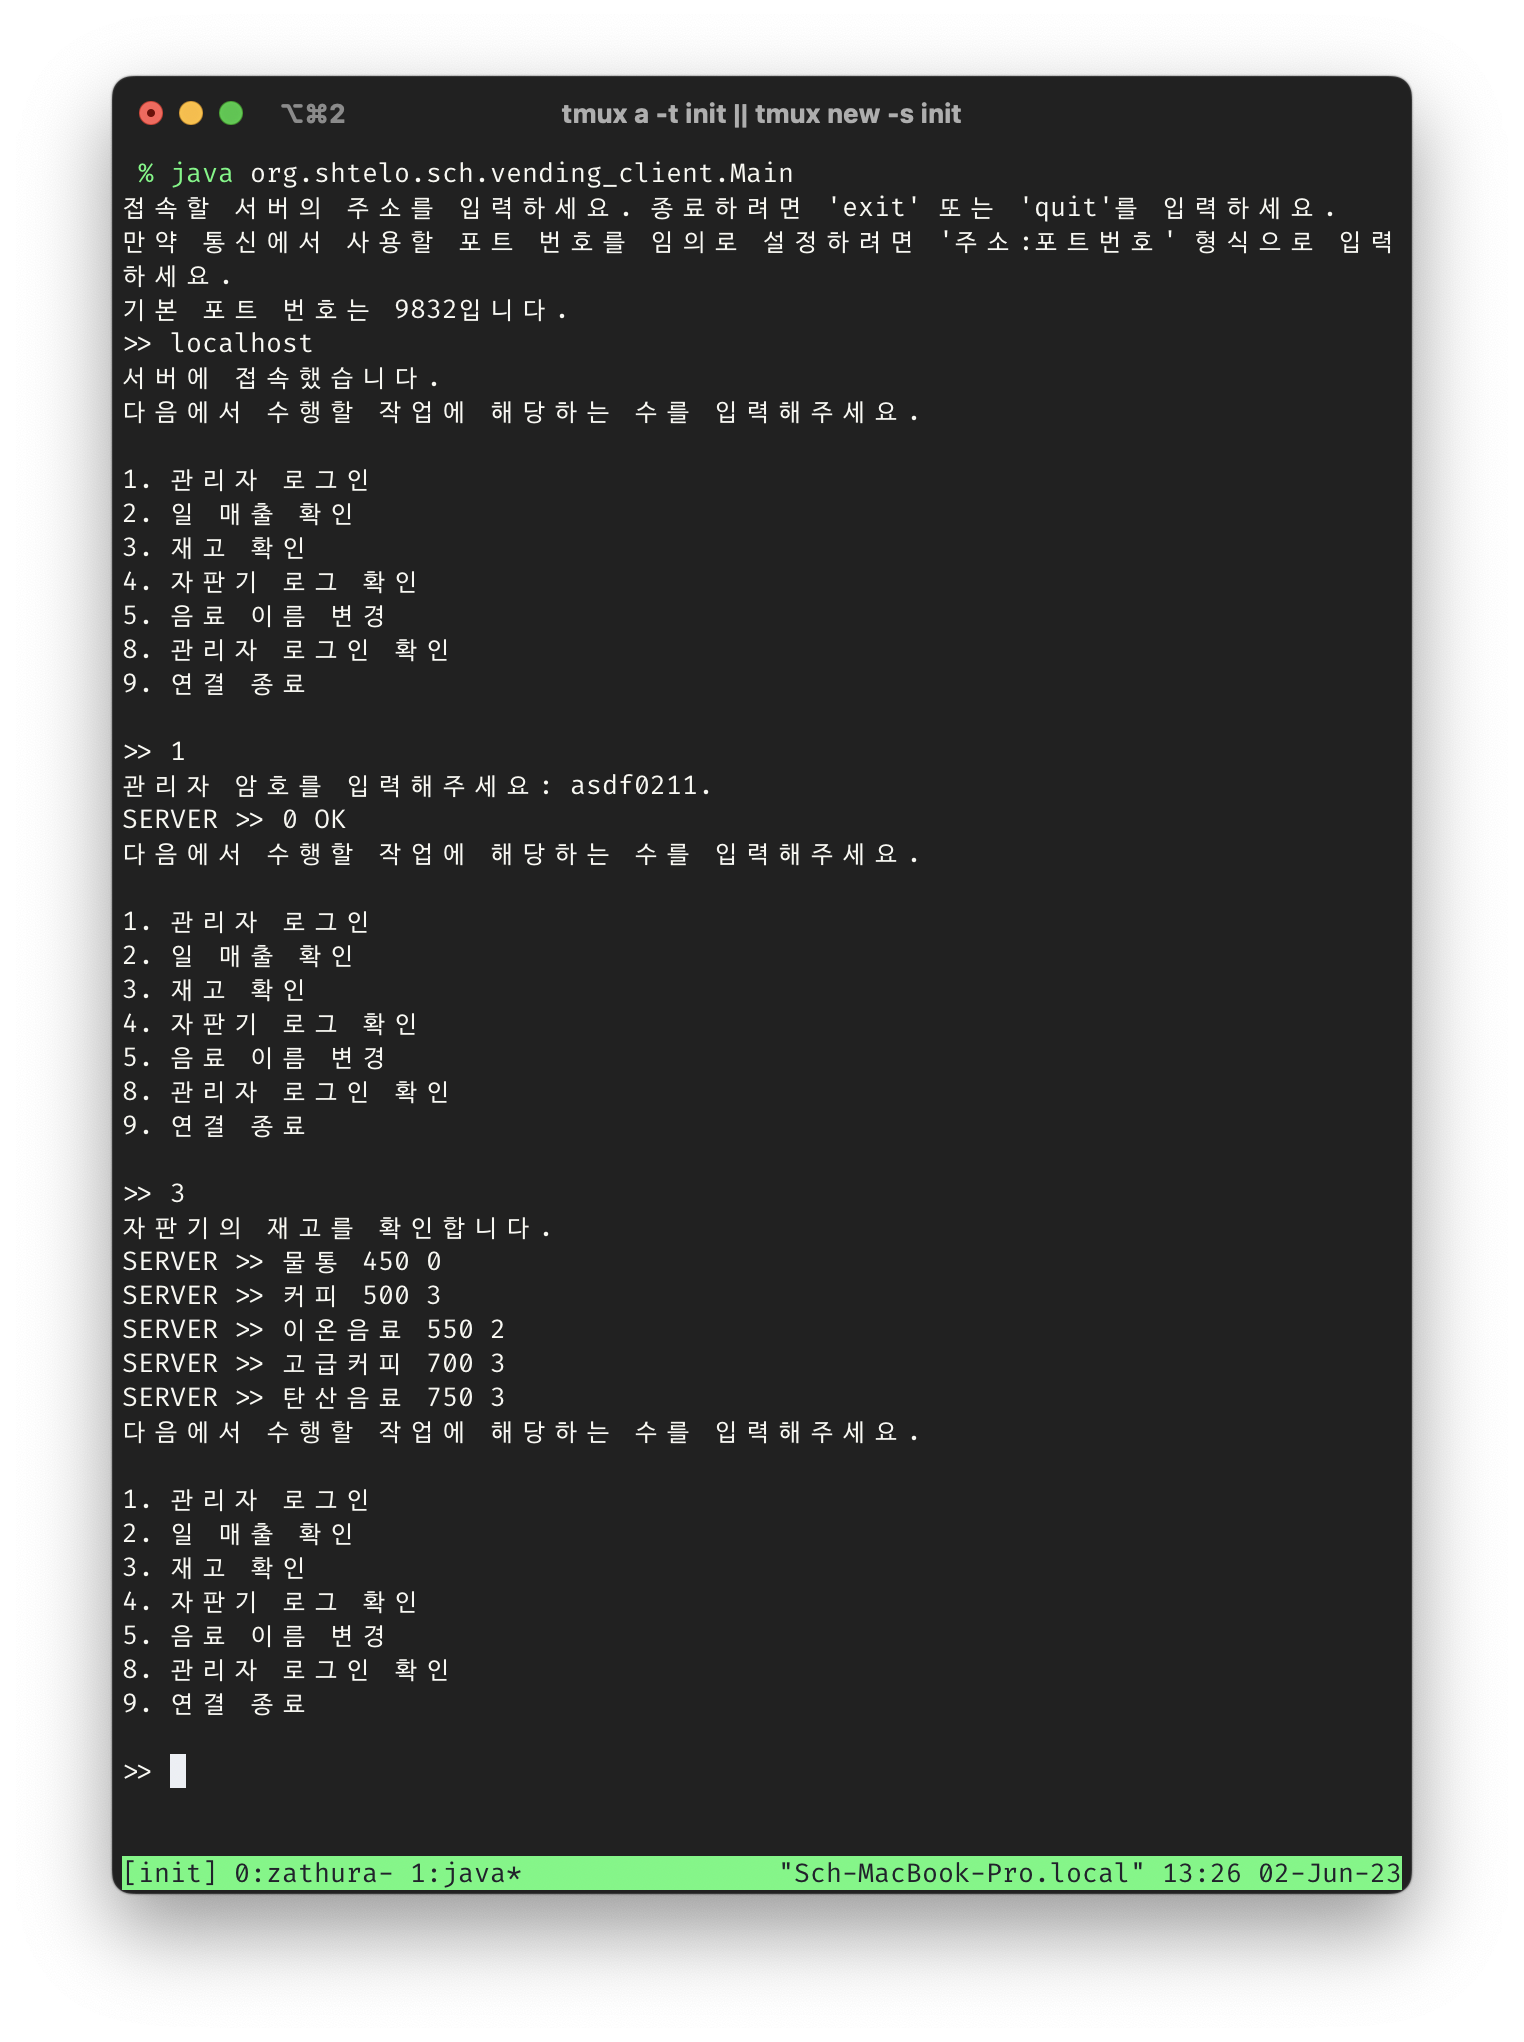
\includegraphics[width=\textwidth]{images/dev-snapshop/0529-client}
        \caption{5월 29일에 구현한 자판기와 클라이언트의 통신}
        \label{fig:0529-client}
    \end{figure}

    \section{설계, 요구사항과의 비교}

    상세 설계에서 나타낸 설계와 실제로 만들어진 프로그램의 내용을 비교하여 추합하자면 다음과 같다.

    화폐 보관함에는 원래 10,000원권까지를 보관할 수 있도록 할 예정이었으나,
    이것이 문제에서 원하는 요구사항을 충족하지 않는 것으로 판단하여 1,000원권까지를 보관할 수 있도록 하였다.

    설계에서는 자판기가 성공적으로 거스름을 수행하지 못했을 때에
    로그를 남겨서 관리자가 직접 잔돈을 처리할 수 있도록 하는 것이 바람직하다고 여겼다.
    하지만 실제로 자판기가 거스름을 성공적으로 처리하지 못했을 때에는
    관리자가 출동하는 것이 아니라 다른 화폐를 투입하여 거스름이 가능한 집합을 만들거나
    그대로 두고 자리를 뜨는 경우가 많다.
    이것을 프로그램에도 반영하여,
    로그를 남기지 않고 사용자가 잔돈 반환이 성공적으로 이루어지지 않았다는 것을
    알 수 있도록 하는 것까지만 구현하였다.

    돈을 넣기 전에 거스를 수 있는 돈이 일정 액수 이하임을 알리는 것을 구현하도록 설계하였으나,
    실제로는 이것을 구현하지 않았다.
    거스를 수 있는 돈이 어떤 종류에 있다는 것을 알아내기 위해서 거스름돈을 계산하는 것이 필요하고,
    이 알고리즘을 구현하는 데에 실패했기 때문에 이 기능을 구현할 수 없었다.

    음료 보관함에 음료가 없을 때에는 현금 투입 이전에 알리는 것을 설계하였으나,
    음료 구매 버튼이 비활성화되어 구매할 수 없게 되는 것과
    거스름 버튼이 구현되어있는 것으로 충분하다고 느껴, 이것을 구현하지 않았다.

    관리자 화면에서는 자판기에 재고가 없을 때에 자판기 재고 목록을 초기화하도록 설계하였으나,
    이것이 자판기 시뮬레이션에 있어 자연스럽지 않은 시나리오라고 판단했다.
    따라서 이 기능을 구현하지 않고, 재고가 없을 때에는 재고가 없는 상태로
    사용자가 음료를 구매할 수 없도록 하였다.
    사용자 경험을 위해서 이러한 설계를 했다고 작성되어 있으나,
    개발하는 시점에 와서 이것이 무엇을 의미하는지 알 수 없어 설계서의 내용을 자세히 기록해야 하겠다는
    생각이 들었다.

    원래는 로그를 JSON 방식으로 저장하여 서버에서 처리할 수 있도록 하는 것이 목표였으나,
    Java에서 JSON을 다루는 방식이 익숙하지 않아서 로그를 일반적인 텍스트 파일로 저장하도록 했다.
    물론 이 경우에도 로그 처리 편의를 위해서 로그를 일정한 방식으로 저장했지만,
    시간 관계상 로그 확인 외의 기능을 구현하지 않았다.

    설계서에는 작성되어있는 내용이 아니지만, 원래는 관리자용 서버가 따로 있고
    자판기가 서버에 접속하여 정보를 저장하는 방식으로 프로그래밍을 진행하려고 했다.
    하지만 서버가 언제나 켜져있는 것이 아니고, 서버를 구현하기 전에 먼저 자판기를 구현했기 때문에
    자판기가 완성되어있는 시점에 서버가 존재하지 않았다.
    자판기에서 발생하는 대부분의 상호작용 정보는 자판기 측에 저장되도록 되었고,
    서버가 제시되었을 때에 이것을 서버에 전송하는 시나리오는
    서버가 켜져있지 않은 경우에 대한 예외 처리를 해야 하는 것이 많아서
    필요 이상의 피로를 유발한다고 판단했다.
    따라서 자판기를 서버로 사용하고 관리자가 클라이언트를 사용하여
    자판기에 접속하는 컨셉을 채택하여 네트워크 통신을 구현하였다.

    \section{느낀 점}

    이번 과제를 하면서 다음 몇 가지 느낀 점이 있었다.

    첫째로, 자판기를 제작하는 것은 생각하는 것보다 복잡하다는 것이다.
    사용자에게 자판기는 돈을 넣고 버튼을 누르면 음료가 나오는 것이 전부이지만,
    실제로 자판기를 구현해보려고 하니 재고 관리나 돈의 투입, 거스름돈 등을 고려해야 하는 것이 많았다.
    우리가 사용하는 자판기는 이것을 모두 고려하여 만들어졌다는 것을 알 수 있었다.

    둘째로, 요구사항을 명확히 하여 알아볼 수 있고 실행 가능한 설계서를 만드는 것이 중요하다는 것이다.
    대부분의 개발은 이렇게 만든 설계서를 바탕으로 이루어지는데,
    설계서가 명확하지 않으면 개발자가 이해하기 어렵고, 개발자가 이해하기 어렵다면
    개발자가 이해한 대로 개발을 하게 되고, 이는 요구사항과 다른 결과물을 만들어 낼 수 있다.
    따라서 요구사항을 명확히 하고, 이를 바탕으로 실행 가능한 설계서를 만드는 것이 중요하다.

    셋째로, 설계서를 완벽하게 따라서 프로그래밍하지 않아도 된다는 것이다.
    설계서는 요구사항을 충족시키기 위해서 어떻게 프로그래밍해야 할지 알려주는 것이지,
    그것이 프로젝트의 목적이 아니다.
    결국 프로그래밍은 주어진 문제를 해결하기 위해서 하는 것이므로,
    문제를 해결할 수 있다면 프로젝트 초반에 만들어놓은 설계서에 완벽히 따를 필요는 없다.
    무엇보다, 설계서를 작성하는 과정에서 문제점이 발생했다면
    그대로 설계서를 따르는 것은 오히려 문제를 더욱 심각하게 만들 수 있다.

    \section{향후 계획}

    일단 이 프로젝트는 과제 제출용으로 진행되었으므로, 과제를 제출하고 나면
    더 이상 진행하지 않을 예정이다.

    이 프로젝트는 내가 만든 프로그램 포트폴리오가 되므로
    특별한 문제가 되지 않는다면
    GitHub에 오픈소스로 공개하여~\cite{github}에서 누구나 볼 수 있도록 할 예정이다.

    \begin{thebibliography}{1}
        \bibitem{github}
        \texttt{junhg0211} (2023), \texttt{vending-machine}, 2023. 6. 5 방문, \url{https://github.com/junhg0211/vending-machine}
    \end{thebibliography}

\end{document}
